% ============================================================
%  VAE Experiments Report
%  Purpose: Detailed documentation of implementation steps,
%           experimental results, and conclusions for VAE models.
%           To be used in a comprehensive comparison with DDPMs.
% ============================================================

\documentclass[12pt, a4paper]{article}

% ── Packages ────────────────────────────────────────────────
\usepackage[T1]{fontenc}
\usepackage[utf8]{inputenc}
\usepackage{lmodern}
\usepackage[margin=2.5cm]{geometry}
\usepackage{graphicx}
\usepackage{float}
\usepackage{subcaption}
\usepackage{booktabs}
\usepackage{array}
\usepackage{tabularx}
\usepackage{amsmath, amssymb}
\usepackage{hyperref}
\usepackage{xcolor}
\usepackage{listings}
\usepackage{caption}
\usepackage{parskip}
\usepackage{titlesec}
\usepackage{fancyhdr}
\usepackage{enumitem}
\usepackage{microtype}
\usepackage{multirow}
\usepackage{tcolorbox}
\tcbuselibrary{breakable, skins}

% ── Hyperref setup ──────────────────────────────────────────
\hypersetup{
    colorlinks = true,
    linkcolor  = blue!60!black,
    citecolor  = green!50!black,
    urlcolor   = blue!70!black,
}

% ── Color palette ───────────────────────────────────────────
\definecolor{codeblue}{RGB}{39,116,174}
\definecolor{codegray}{RGB}{240,240,240}
\definecolor{accent}{RGB}{0,90,160}
\definecolor{boxframe}{RGB}{0,90,160}
\definecolor{boxbg}{RGB}{235,245,255}

% ── Section title formatting ────────────────────────────────
\titleformat{\section}[block]
  {\Large\bfseries\color{accent}}
  {\thesection}{1em}{}[\titlerule]

\titleformat{\subsection}[block]
  {\large\bfseries\color{accent!80!black}}
  {\thesubsection}{1em}{}

\titleformat{\subsubsection}[block]
  {\normalsize\bfseries}
  {\thesubsubsection}{1em}{}

% ── Code listing style ──────────────────────────────────────
\lstset{
    backgroundcolor  = \color{codegray},
    basicstyle       = \ttfamily\small,
    keywordstyle     = \color{codeblue}\bfseries,
    commentstyle     = \color{gray}\itshape,
    stringstyle      = \color{red!60!black},
    numbers          = left,
    numberstyle      = \tiny\color{gray},
    numbersep        = 8pt,
    frame            = single,
    rulecolor        = \color{gray!40},
    breaklines       = true,
    captionpos       = b,
    tabsize          = 4,
    showstringspaces = false,
}

% ── Config box ──────────────────────────────────────────────
\newtcolorbox{configbox}[1][]{
    enhanced,
    colback   = boxbg,
    colframe  = boxframe,
    fonttitle = \bfseries,
    title     = {#1},
    breakable,
    arc       = 3pt,
}

% ── Header / Footer ─────────────────────────────────────────
\pagestyle{fancy}
\fancyhf{}
\rhead{\small VAE Experiments Report}
\lhead{\small Generative Models — VAEs vs.\ DDPMs}
\cfoot{\thepage}
\renewcommand{\headrulewidth}{0.4pt}

% ── Graphics path ───────────────────────────────────────────
% Place all exported figures in the same folder as this .tex file,
% or adjust the path below:
\graphicspath{{./figures/}}

% ============================================================
\begin{document}

% ── Title page ──────────────────────────────────────────────
\begin{titlepage}
    \centering
    \vspace*{2cm}
    {\Huge\bfseries\color{accent} Variational Autoencoders\\[0.4em]
     \Large Experimental Report}\\[1em]
    \rule{\linewidth}{0.6pt}\\[1.5em]
    {\large\itshape
     Detailed documentation of implementation steps, experimental results,
     and conclusions for VAE-based generative models.\\[0.6em]
     Part of a comprehensive comparison with Denoising Diffusion
     Probabilistic Models (DDPMs).}\\[3em]
    {\large \today}
    \vfill
    \begin{tcolorbox}[colback=boxbg, colframe=boxframe, width=0.85\linewidth,
                      arc=4pt, fonttitle=\bfseries,
                      title={Report Structure}]
        \begin{itemize}[leftmargin=1.2em]
            \item \textbf{Part I — Background:} Theory of VAEs and model architecture
            \item \textbf{Part II — Experimental Setup:} Fixed hyperparameters and dataset
            \item \textbf{Part III — Experiments:} Per-experiment results, analysis, and
                  figures (losses, samples, reconstructions, latent spaces)
            \item \textbf{Part IV — Conclusions:} Summary of findings and key differences
        \end{itemize}
    \end{tcolorbox}
\end{titlepage}

% ── Table of contents ───────────────────────────────────────
\tableofcontents
\newpage

% ============================================================
\section{Introduction}
\label{sec:intro}

This report documents a systematic experimental study of
\textbf{Variational Autoencoders (VAEs)} applied to image generation.
Each experiment targets a specific design choice — conditioning
strategy, attention mechanism, perceptual loss, or capacity — and
evaluates its effect on generation quality, reconstruction fidelity,
and latent-space structure.

The document is designed to serve as one half of a broader
\textbf{comparative analysis between VAEs and Denoising Diffusion
Probabilistic Models (DDPMs)}, enabling an apples-to-apples comparison
of two dominant paradigms in deep generative modelling.

\subsection{Purpose of the Comparison}

VAEs and DDPMs represent fundamentally different inductive biases:

\begin{itemize}
    \item \textbf{VAEs} learn an explicit, amortised posterior
          $q_\phi(\mathbf{z} | \mathbf{x})$ and optimise a tractable
          Evidence Lower Bound (ELBO), trading reconstruction sharpness
          for a structured, continuous latent space.

    \item \textbf{DDPMs} learn to reverse a fixed Markov diffusion
          process, achieving high sample quality at the cost of slow,
          iterative inference.
\end{itemize}

Both model families are trained on the \textbf{same architectural
backbone}, the same dataset, and the same fixed hyperparameters, so
that differences in metrics reflect the generative paradigm rather
than implementation disparity.

% ============================================================
\section{Background: Variational Autoencoders}
\label{sec:background}

% ── Placeholder ─────────────────────────────────────────────
\begin{tcolorbox}[colback=yellow!8, colframe=orange!60!black,
                  fonttitle=\bfseries, title={Content placeholder}]
This section will contain:
\begin{itemize}
    \item A concise derivation of the ELBO objective
    \item The reparameterisation trick
    \item KL-divergence regularisation and its role
    \item Perceptual / feature-matching losses
    \item Conditional generation strategies (class embeddings,
          AdaGN, concatenation)
\end{itemize}
\end{tcolorbox}

\subsection{Model Architecture}
\label{subsec:architecture}

% ── Placeholder ─────────────────────────────────────────────
\begin{tcolorbox}[colback=yellow!8, colframe=orange!60!black,
                  fonttitle=\bfseries, title={Content placeholder}]
This section will contain:
\begin{itemize}
    \item Encoder–decoder design (U-Net style with residual blocks)
    \item Channel multiplier schedule
    \item Attention insertion points
    \item Conditioning injection: AdaGN vs.\ channel-concatenation
    \item Comparison diagram vs.\ DDPM denoiser architecture
\end{itemize}
\end{tcolorbox}

% ============================================================
\section{Experimental Setup}
\label{sec:setup}

\subsection{Dataset}
All experiments use a 10-class image dataset with resolution
$32 \times 32$ pixels.

\subsection{Fixed Hyperparameters}
\label{subsec:fixed-hp}

The following hyperparameters are held constant across \emph{all}
experiments to ensure fair comparison:

\begin{configbox}[Fixed Hyperparameters (all experiments)]
\begin{lstlisting}[language=Python, numbers=none]
{
    "image_size"    : 32,       # Input / output resolution (px)
    "num_classes"   : 10,       # Number of conditioning classes
    "latent_dim"    : 128,      # Dimensionality of latent space z
    "base_channels" : 64,       # Feature-map width at first encoder level
    "channel_mults" : [1, 2, 4],# Channel multipliers per resolution level
    "num_res_blocks": 2,        # Residual blocks per resolution level
    "batch_size"    : 32,       # Training batch size
    "lr"            : 0.0002,   # Adam learning rate
}
\end{lstlisting}
\end{configbox}

\subsection{Model Variants}
\label{subsec:exp1-variants}

\begin{itemize}
	\item \textbf{VAE} — Vanilla VAE with reconstruction + KL loss only.
	\item \textbf{PercepVAE} — VAE augmented with a perceptual
	(feature-matching) loss.
	\item \textbf{cVAE-AdaGN} — Conditional VAE using Adaptive Group
	Normalisation to inject class information.
	\item \textbf{cVAE-Concat} — Conditional VAE using channel
	concatenation of the class embedding.
\end{itemize}

\subsection{Evaluation Metrics}
\label{subsec:metrics}

\begin{description}[leftmargin=2em]
    \item[\textbf{FID}] Fréchet Inception Distance — measures the
          distributional gap between real and generated images in
          Inception feature space. \emph{Lower is better.}

    \item[\textbf{IS (Inception Score)}] Evaluates both the quality and
          diversity of generated images. Reported as mean $\pm$ standard
          deviation over multiple splits. \emph{Higher is better.}
\end{description}

% ============================================================
\section{Experiment 1}
\label{sec:exp1}

\subsection{Motivation}
\label{subsec:exp1-motivation}

The first experiment establishes the \textbf{baseline} performance of
four VAE variants that differ in their conditioning and loss strategy,
without self-attention. This provides a reference point for subsequent
ablations.

\subsection{Hyperparameters}
\label{subsec:exp1-hp}

\begin{configbox}[Experiment 1 — Variable Hyperparameters]
\begin{lstlisting}[language=Python, numbers=none]
{
    "epochs"        : 50,
    "kl_weight"     : 0.001,   # Weight on KL-divergence term
    "percep_weight" : 0.1,     # Weight on perceptual loss
    "use_attention" : false,   # Self-attention disabled
    "attn_heads"    : 1,
}
\end{lstlisting}
\end{configbox}



\subsection{Evaluation Results}
\label{subsec:exp1-results}

\begin{table}[H]
    \centering
    \caption{Experiment 1 — Quantitative evaluation (FID and IS).
             FID: lower is better; IS: higher is better.}
    \label{tab:exp1-metrics}
    \begin{tabular}{lccc}
        \toprule
        \textbf{Model} & \textbf{FID}~$\downarrow$
                        & \textbf{IS mean}~$\uparrow$
                        & \textbf{IS std} \\
        \midrule
        VAE            & 195.33 & 2.98 & 0.09 \\
        PercepVAE      & 174.83 & 2.93 & 0.08 \\
        cVAE-AdaGN     & 171.04 & 3.16 & 0.10 \\
        cVAE-Concat    & 163.23 & 3.54 & 0.10 \\
        \bottomrule
    \end{tabular}
\end{table}

\subsection{Training Dynamics}
\label{subsec:exp1-training}

\begin{figure}[H]
    \centering
    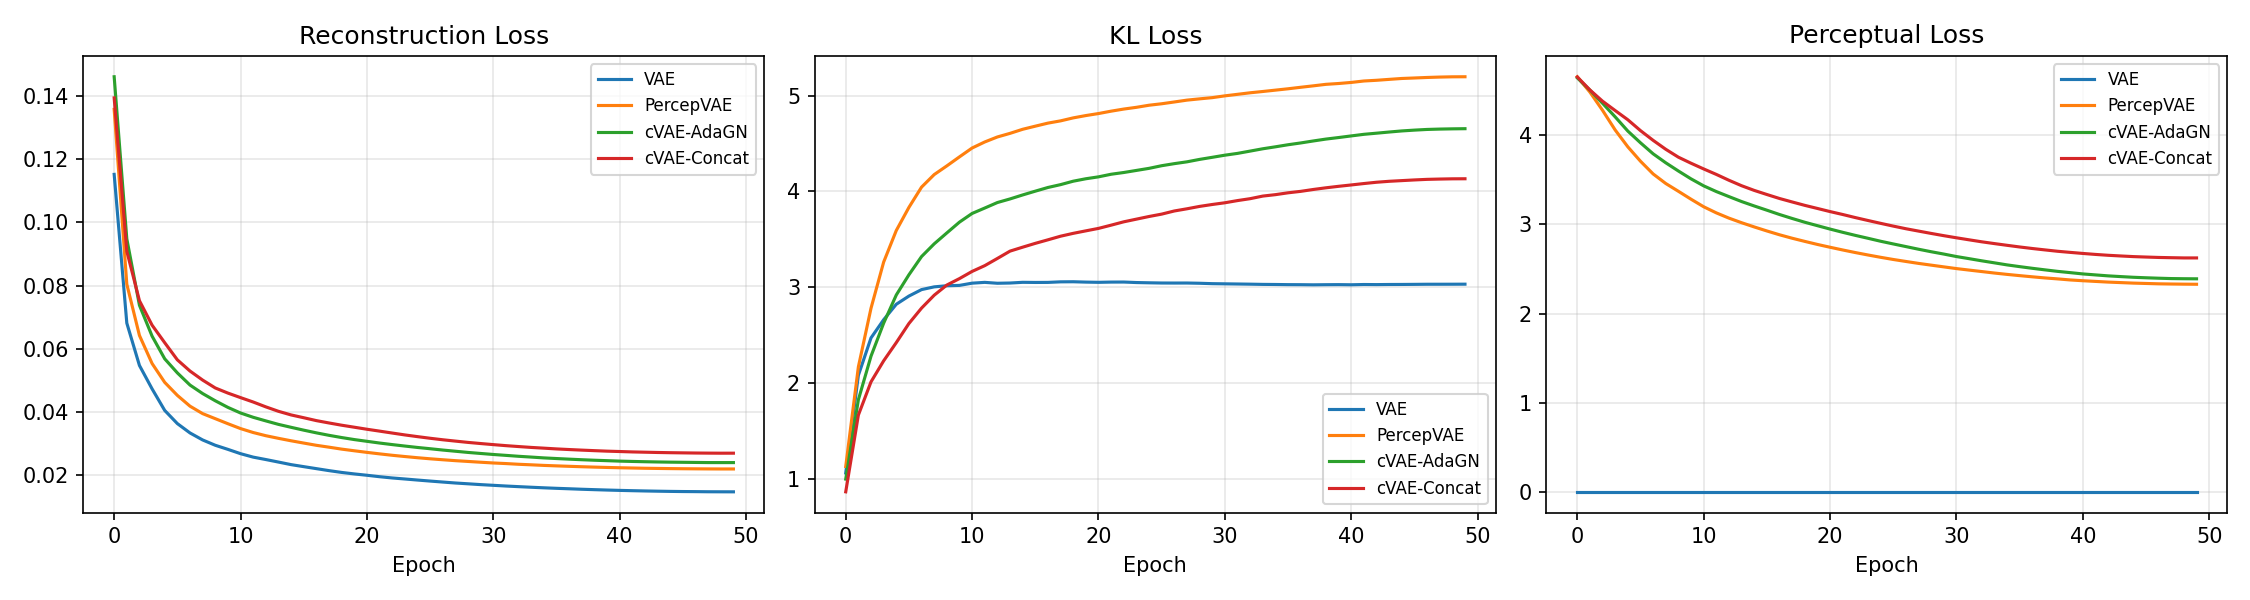
\includegraphics[width=\linewidth]{./exp_1/training_curves.png}
    \caption{Experiment 1 — Training loss curves for all four VAE
             variants. The plot shows the evolution of the total
             loss, reconstruction term, and KL-divergence term over
             50 epochs.}
    \label{fig:exp1-losses}
\end{figure}

\subsection{Qualitative Results}
\label{subsec:exp1-qual}

\subsubsection{Random Samples}

\begin{figure}[H]
    \centering
    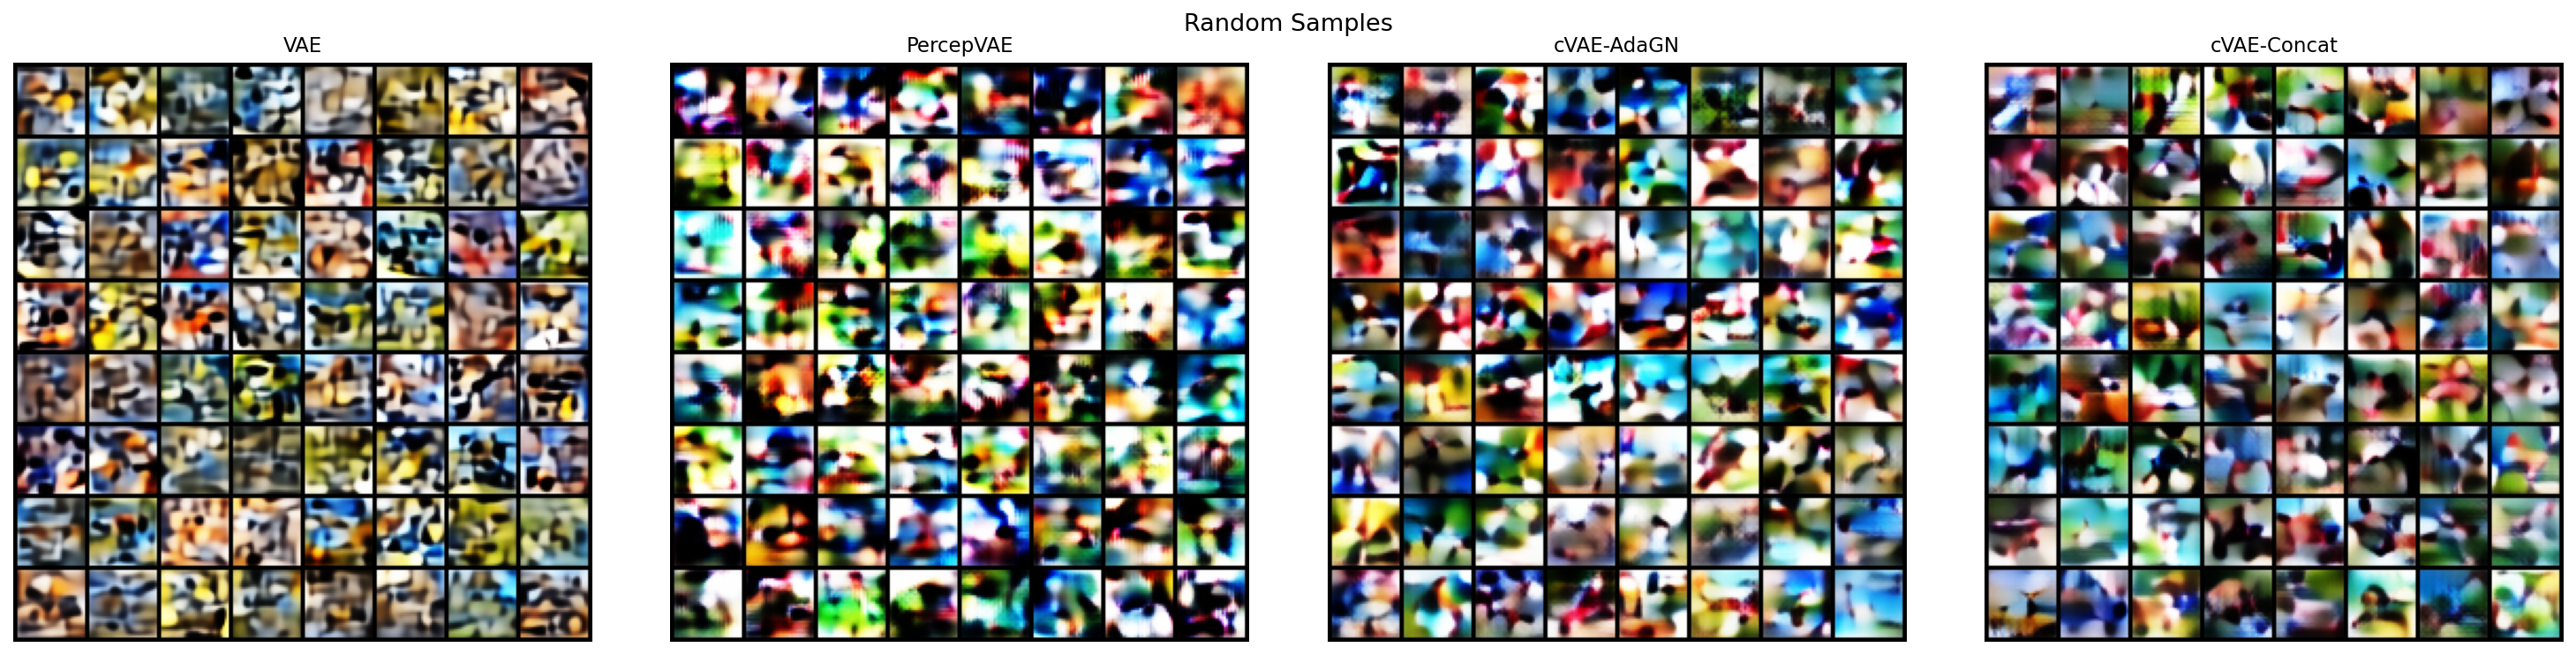
\includegraphics[width=\linewidth]{./exp_1/samples.png}
    \caption{Experiment 1 — Randomly sampled images generated by
             decoding latent vectors $\mathbf{z} \sim \mathcal{N}(0,I)$.}
    \label{fig:exp1-samples}
\end{figure}

\subsubsection{Reconstructions}

\begin{figure}[H]
    \centering
    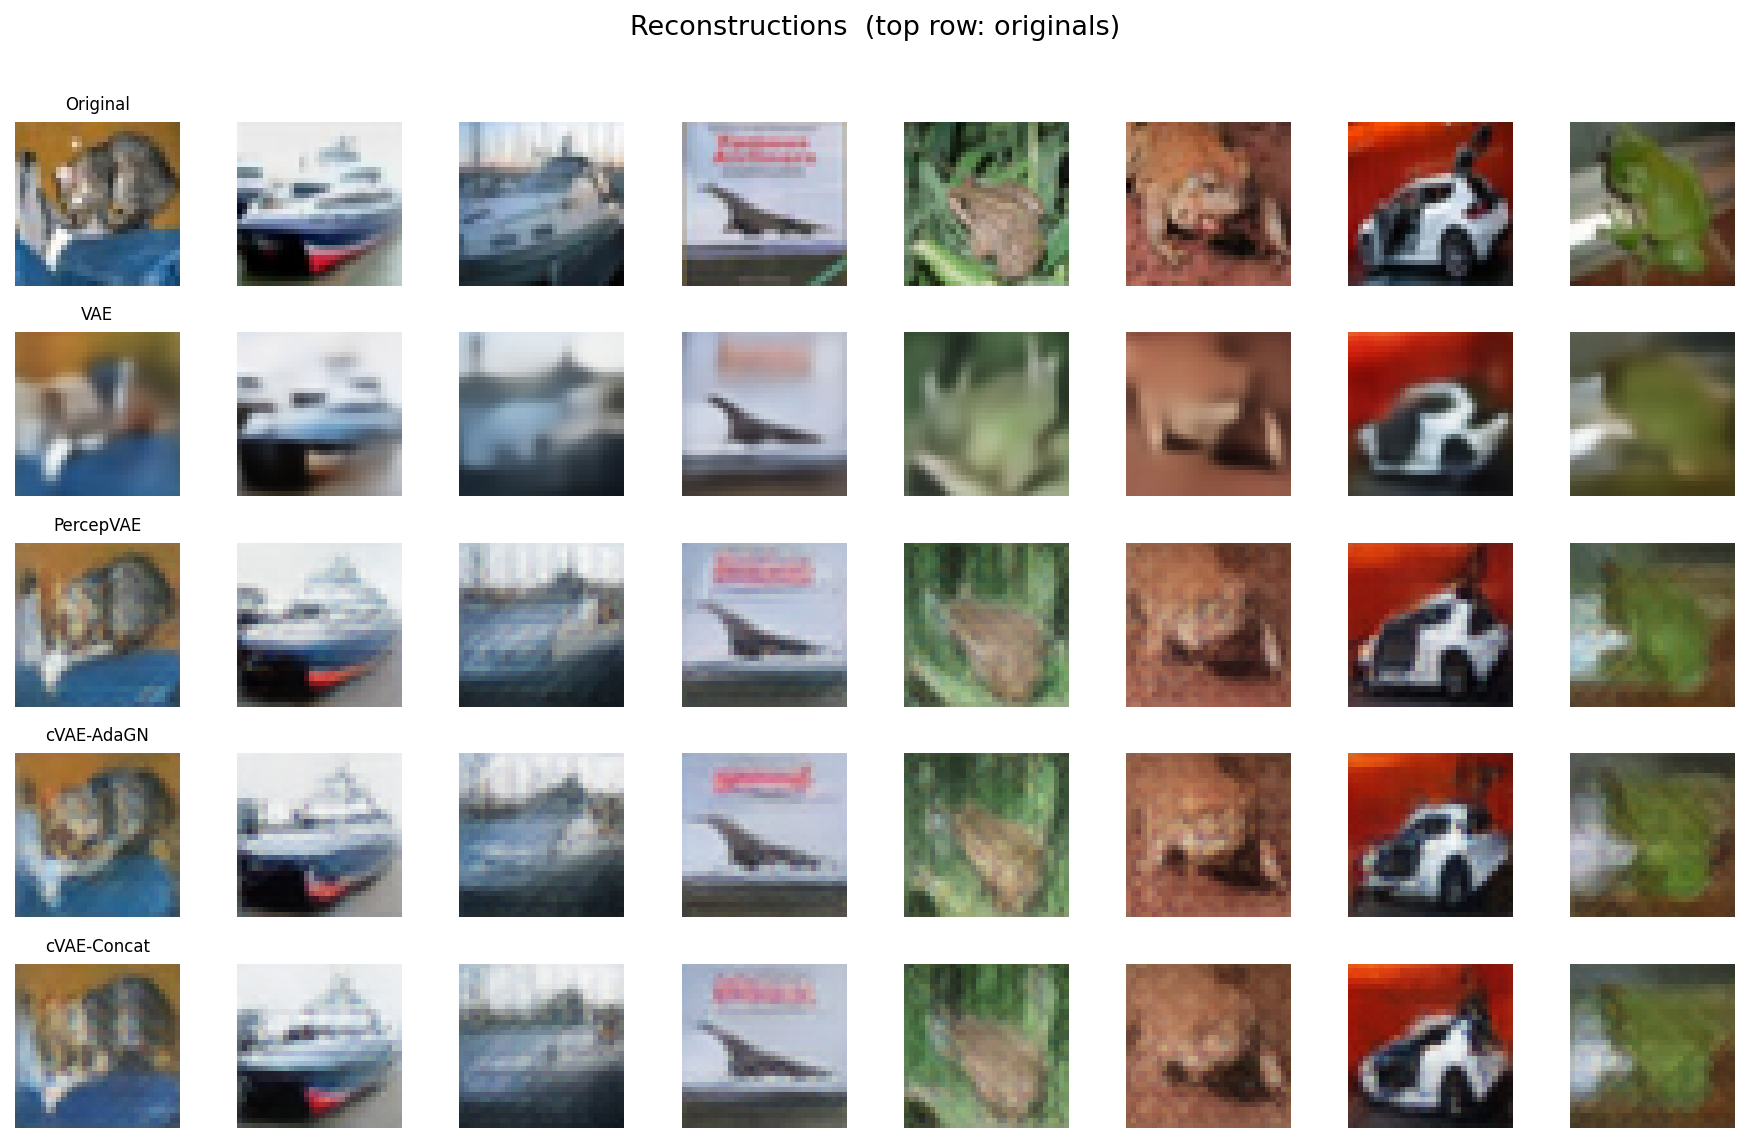
\includegraphics[width=\linewidth]{./exp_1/reconstructions.png}
    \caption{Experiment 1 — Input images (top row) and their
             reconstructions (bottom row). Reconstruction quality is
             noticeably better than free generation, reflecting the
             encoder's ability to infer informative posterior means.}
    \label{fig:exp1-recon}
\end{figure}

\subsubsection{Latent-Space Interpolations}

\begin{figure}[H]
    \centering
    \begin{subfigure}[t]{0.48\linewidth}
        \centering
        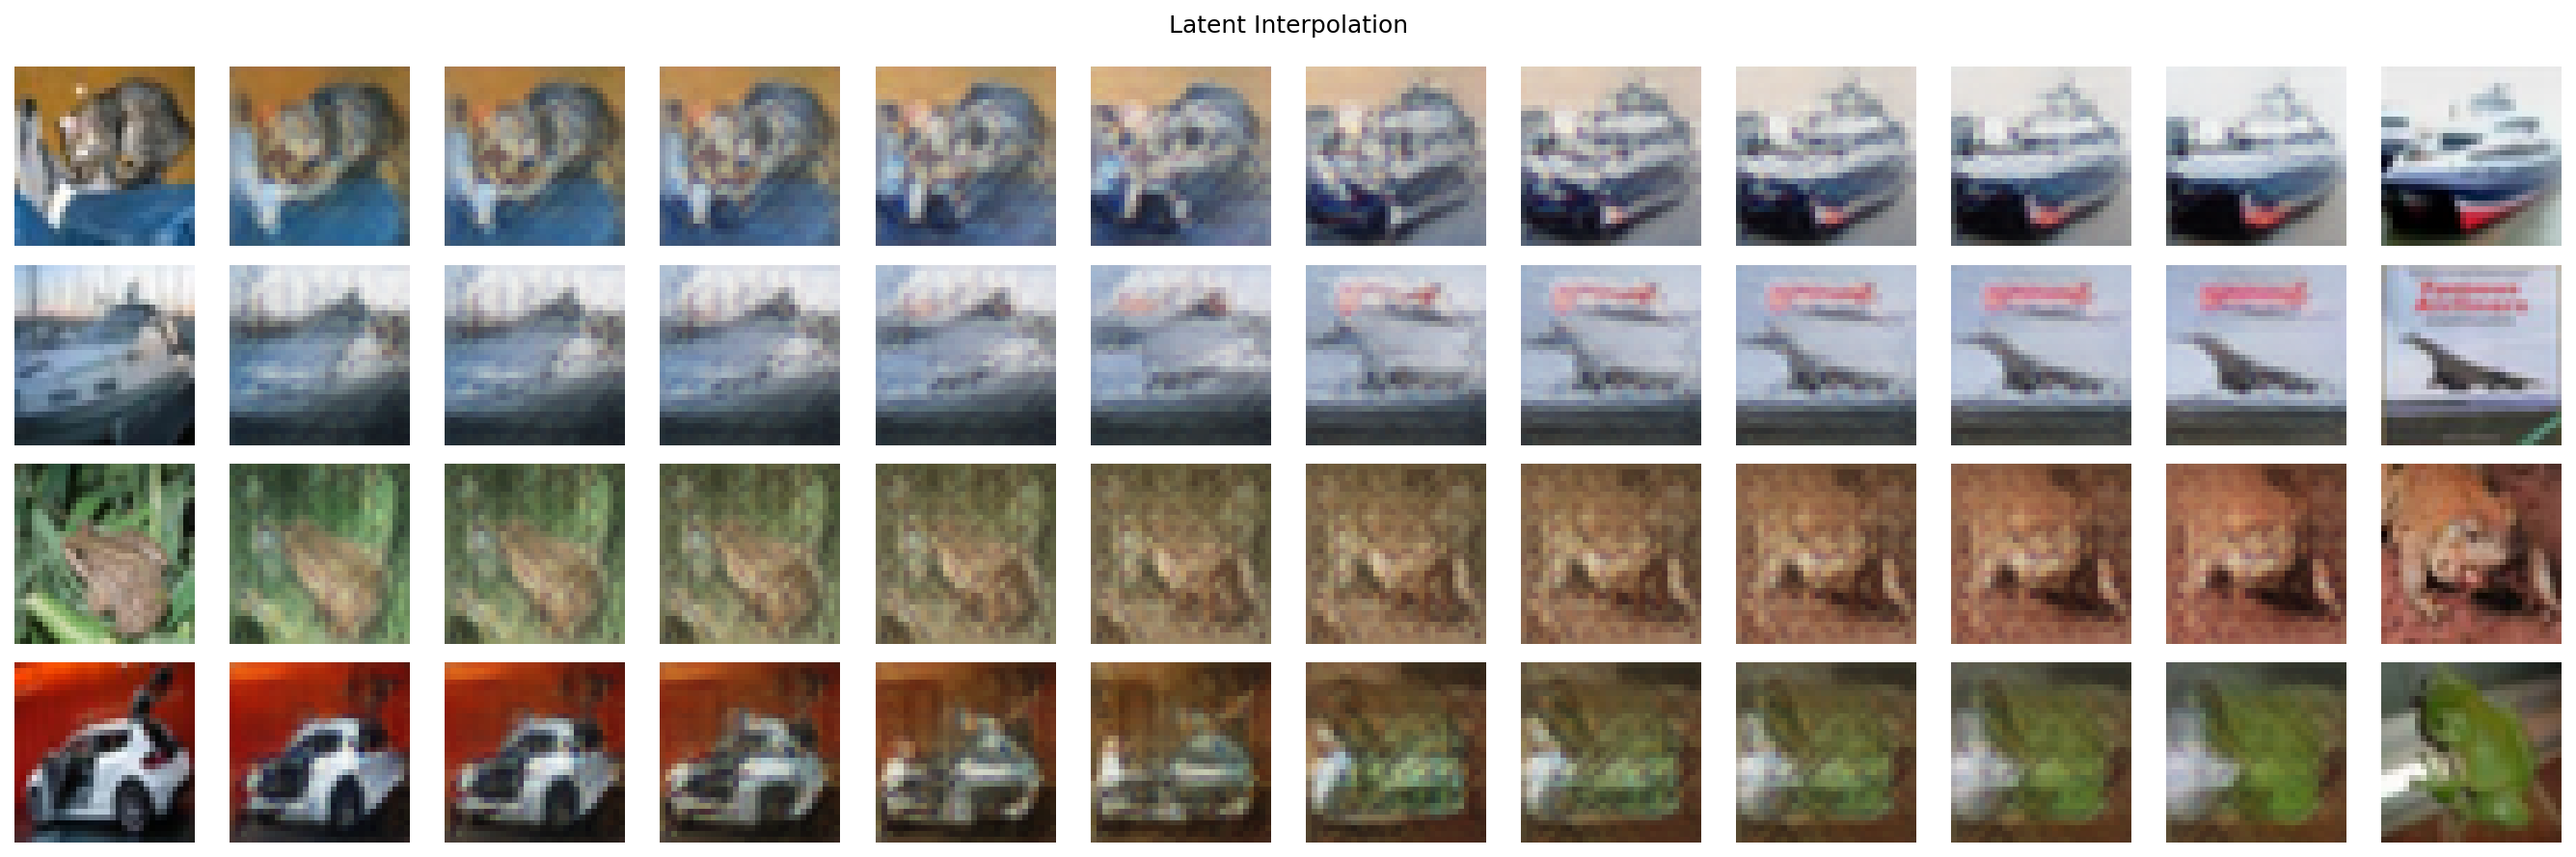
\includegraphics[width=\linewidth]{./exp_1/interp_cvae.png}
        \caption{Interpolation For CVAE-AdaGN.}
    \end{subfigure}
    \hfill
    \begin{subfigure}[t]{0.48\linewidth}
        \centering
        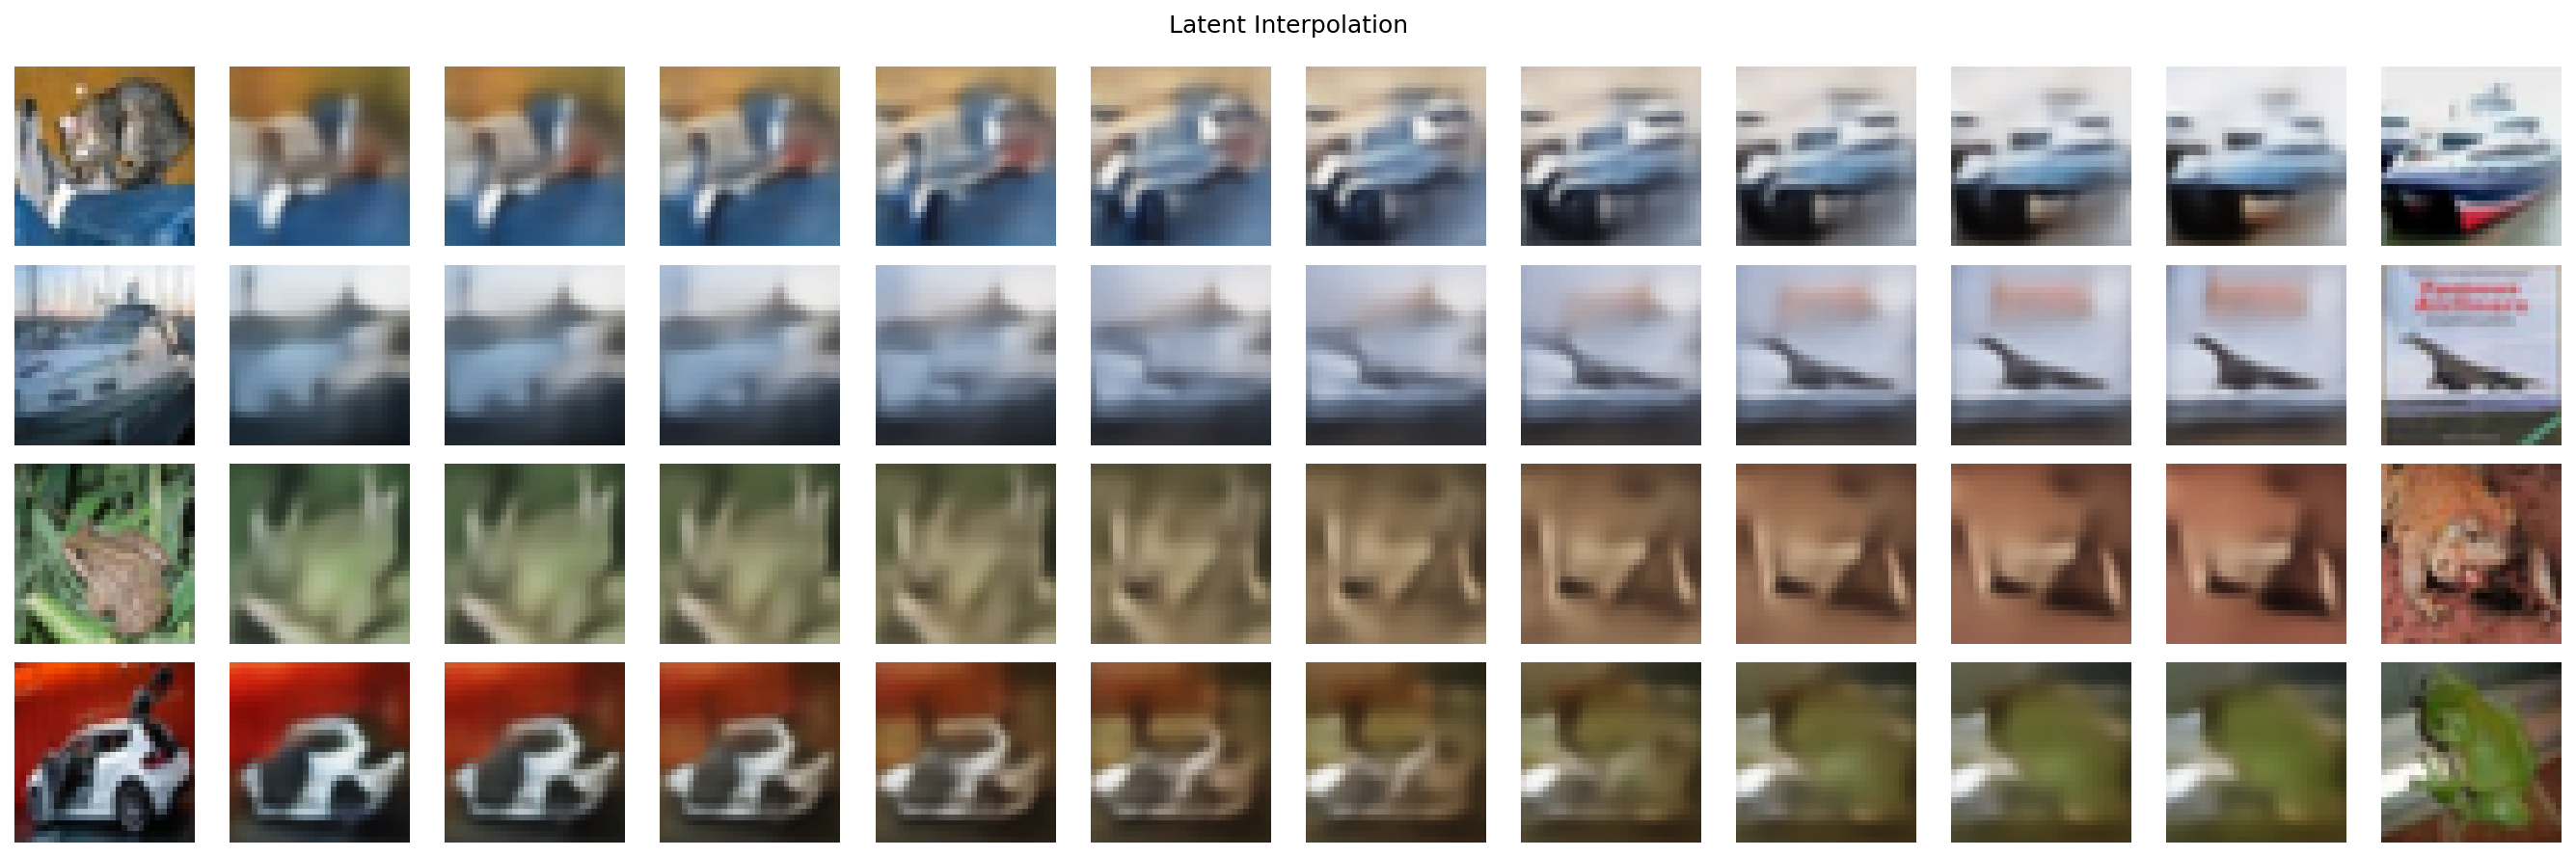
\includegraphics[width=\linewidth]{./exp_1/interp_vae.png}
        \caption{Interpolation For Vanilla VAE.}
    \end{subfigure}
    \caption{Experiment 1 — linear interpolation
             between pairs of encoded images in latent space.}
    \label{fig:exp1-interp}
\end{figure}

\subsubsection{Latent-Space Visualisation}

\begin{figure}[H]
    \centering
    \begin{subfigure}[t]{0.31\linewidth}
        \centering
        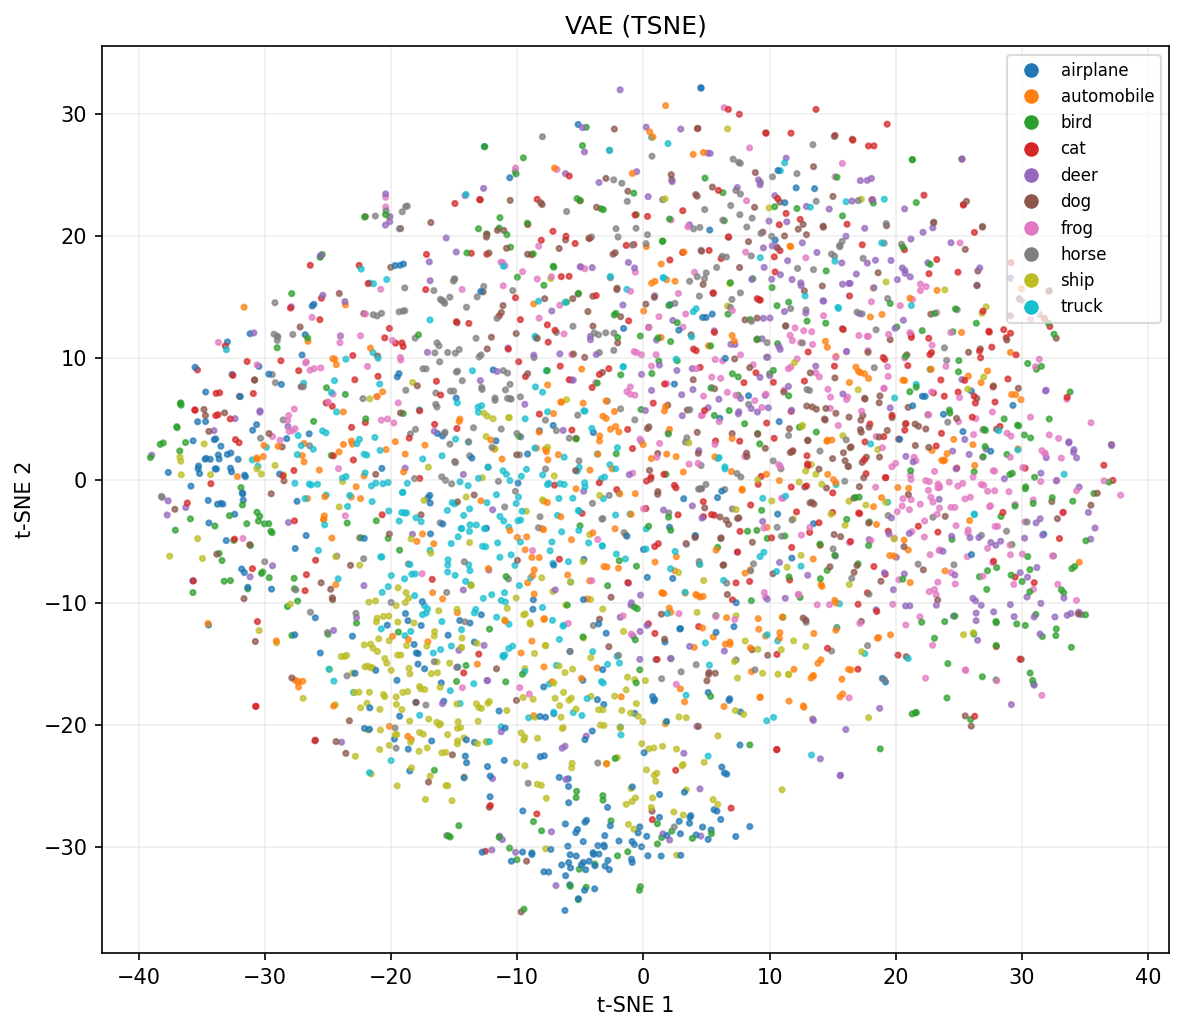
\includegraphics[width=\linewidth]{./exp_1/latent_vae.png}
        \caption{VAE}
    \end{subfigure}
    \hfill
    \begin{subfigure}[t]{0.31\linewidth}
        \centering
        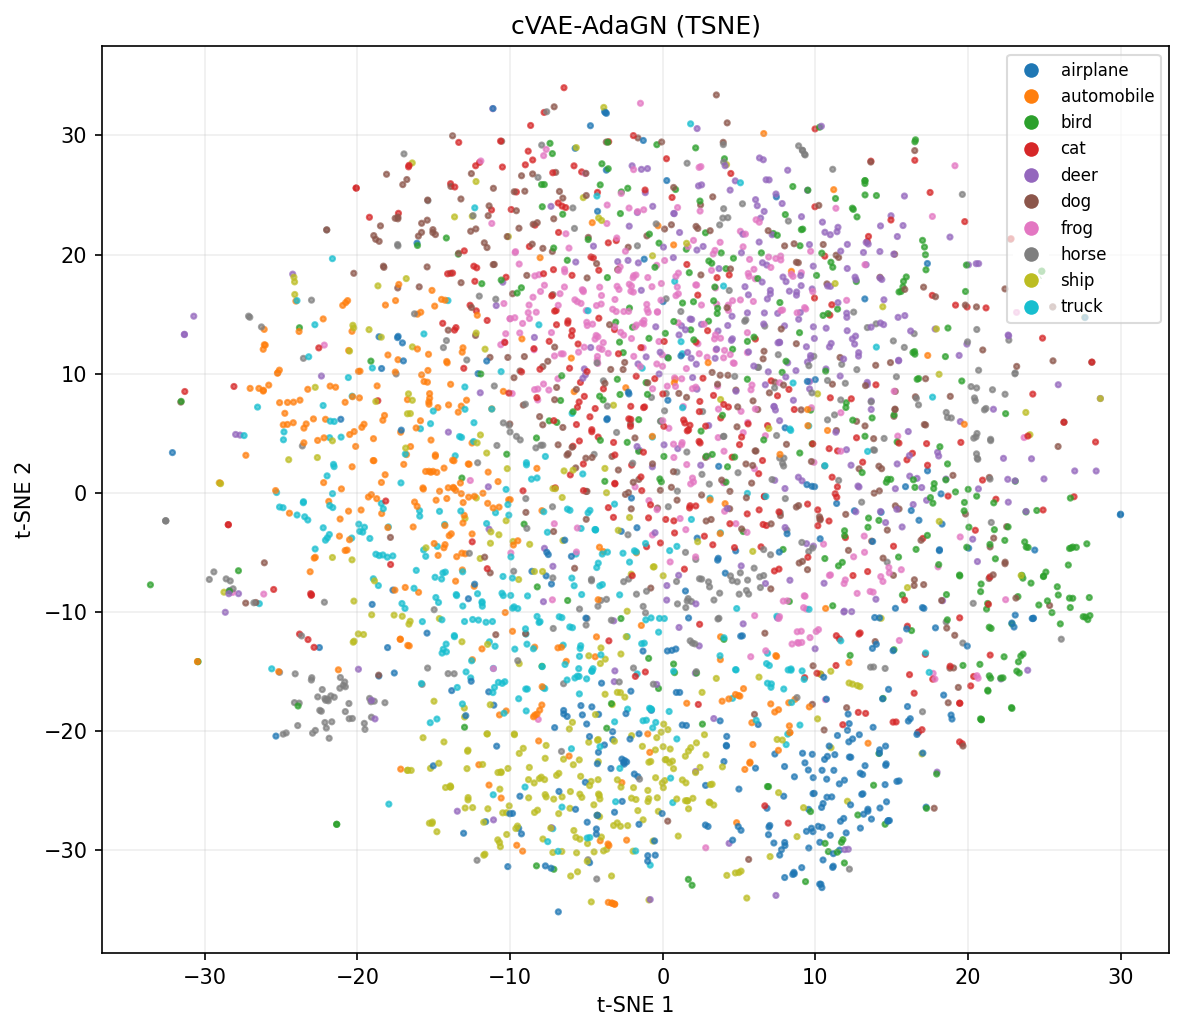
\includegraphics[width=\linewidth]{./exp_1/latent_cvae_adagn.png}
        \caption{cVAE-AdaGN}
    \end{subfigure}
    \hfill
    \begin{subfigure}[t]{0.31\linewidth}
        \centering
        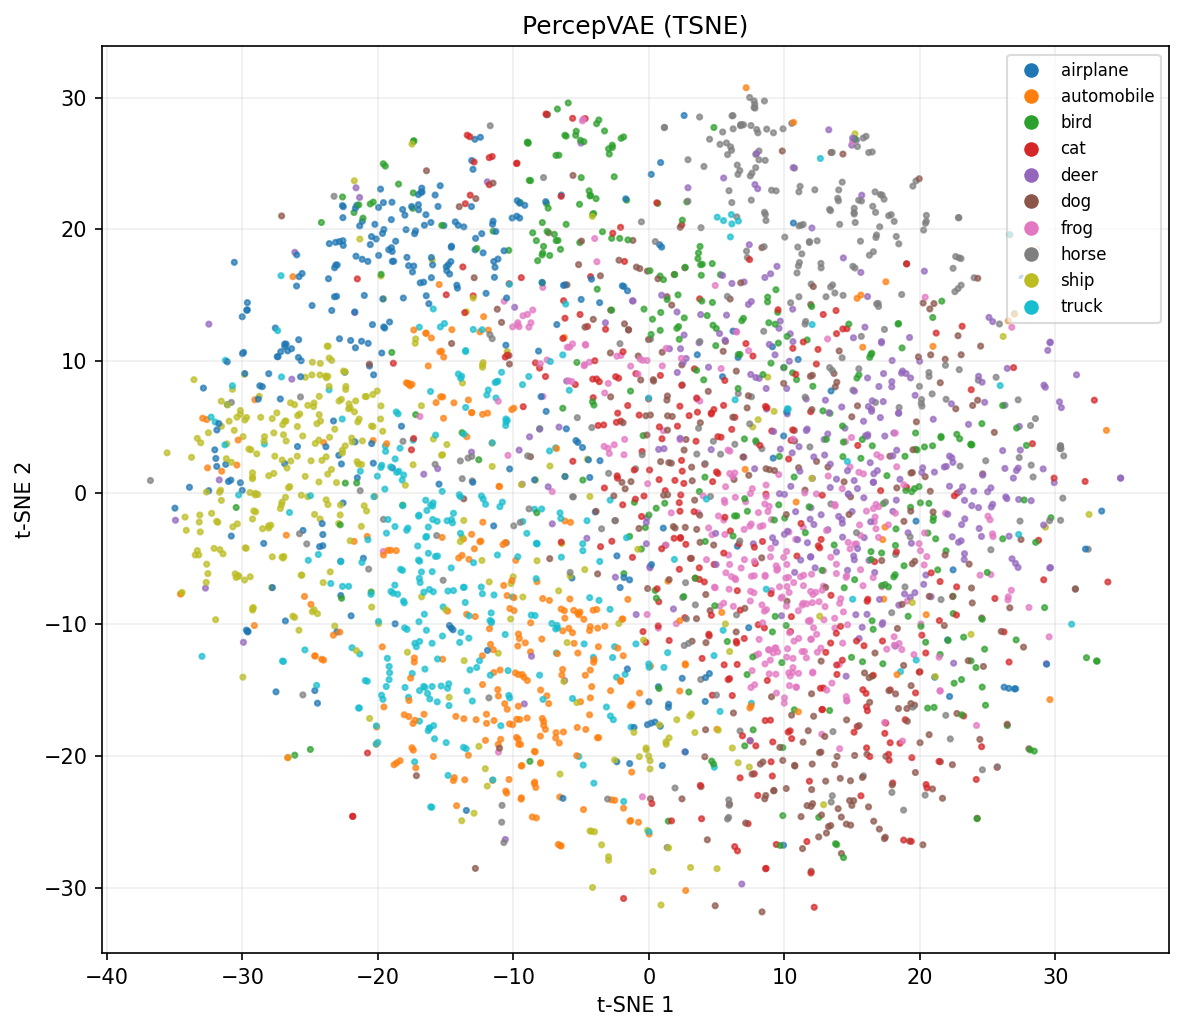
\includegraphics[width=\linewidth]{./exp_1/latent_percepvae.png}
        \caption{Perceptual VAE}
    \end{subfigure}
    \caption{Experiment 1 — 2-D t-SNE projections of the latent
             space, coloured by class label.  Tighter, better-separated
             clusters indicate that the model has learned
             class-discriminative structure in $\mathbf{z}$.}
    \label{fig:exp1-latent}
\end{figure}

\subsection{Analysis and Observations}
\label{subsec:exp1-analysis}

\begin{itemize}
    \item \textbf{Conditioning is decisive.} Both cVAE variants
          outperform the unconditional baselines by a substantial margin,
          with cVAE-Concat achieving the lowest FID (163.23) and the
          highest IS (3.54).

    \item \textbf{Perceptual loss provides moderate benefit.}
          PercepVAE reduces FID by $\approx$20 points vs.\ the vanilla
          VAE, but its IS slightly decreases, suggesting that perceptual
          regularisation may introduce a diversity-quality trade-off.

    \item \textbf{AdaGN vs.\ Concat.} cVAE-Concat outperforms
          cVAE-AdaGN on both FID and IS, indicating that direct feature
          concatenation is a more effective conditioning mechanism than
          normalisation-layer modulation at this scale.

    \item \textbf{Reconstruction vs.\ generation gap.}
          Reconstruction quality is visually good (see
          Figure~\ref{fig:exp1-recon}), while free-sampling quality
          remains limited (Figure~\ref{fig:exp1-samples}). This
          posterior-prior gap is a well-known VAE limitation.

    \item \textbf{Latent structure.} The t-SNE plots
          (Figure~\ref{fig:exp1-latent}) show that conditional model
          form tighter, more separable clusters, consistent with
          improved IS scores.
\end{itemize}



% ============================================================
\section{Experiment 2}
\label{sec:exp1}

\subsection{Motivation}
\label{subsec:exp1-motivation}

The first experiment establishes the \textbf{baseline} performance of
four VAE variants that differ in their conditioning and loss strategy,
without self-attention. This provides a reference point for subsequent
ablations.

\subsection{Hyperparameters}
\label{subsec:exp1-hp}

\begin{configbox}[Experiment 1 — Variable Hyperparameters]
	\begin{lstlisting}[language=Python, numbers=none]
		{
			"epochs"        : 50,
			"kl_weight"     : 1.0,   # Weight on KL-divergence term
			"percep_weight" : 0.1,     # Weight on perceptual loss
			"use_attention" : false,   # Self-attention disabled
			"attn_heads"    : 1,
		}
	\end{lstlisting}
\end{configbox}



\subsection{Evaluation Results}
\label{subsec:exp1-results}

\begin{table}[H]
	\centering
	\caption{Experiment 1 — Quantitative evaluation (FID and IS).
		FID: lower is better; IS: higher is better.}
	\label{tab:exp1-metrics}
	\begin{tabular}{lccc}
		\toprule
		\textbf{Model} & \textbf{FID}~$\downarrow$
		& \textbf{IS mean}~$\uparrow$
		& \textbf{IS std} \\
		\midrule
		VAE            & 326.79 & 1.69 & 0.03 \\
		PercepVAE      & 276.51 & 2.22 & 0.06 \\
		cVAE-AdaGN     & 394.40 & 2.03 & 0.03 \\
		cVAE-Concat    & 193.62 & 3.41 & 0.12 \\
		\bottomrule
	\end{tabular}
\end{table}

\subsection{Training Dynamics}
\label{subsec:exp1-training}

\begin{figure}[H]
	\centering
	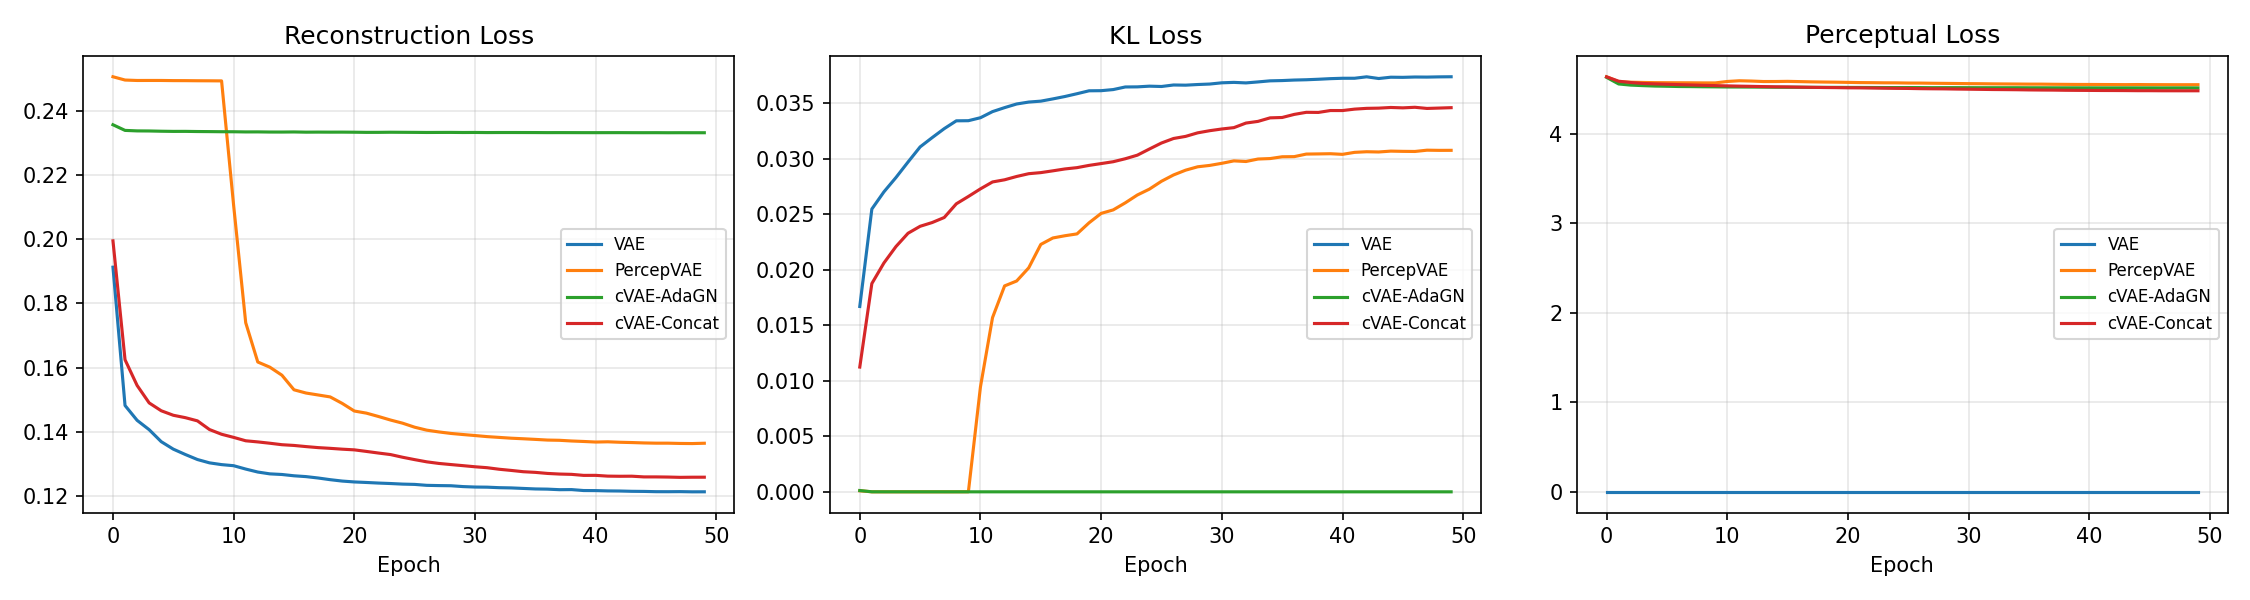
\includegraphics[width=\linewidth]{./with_KL_equals_1/training_curves.png}
	\caption{Experiment 1 — Training loss curves for all four VAE
		variants. The plot shows the evolution of the total
		loss, reconstruction term, and KL-divergence term over
		50 epochs.}
	\label{fig:exp1-losses}
\end{figure}

\subsection{Qualitative Results}
\label{subsec:exp1-qual}

\subsubsection{Random Samples}

\begin{figure}[H]
	\centering
	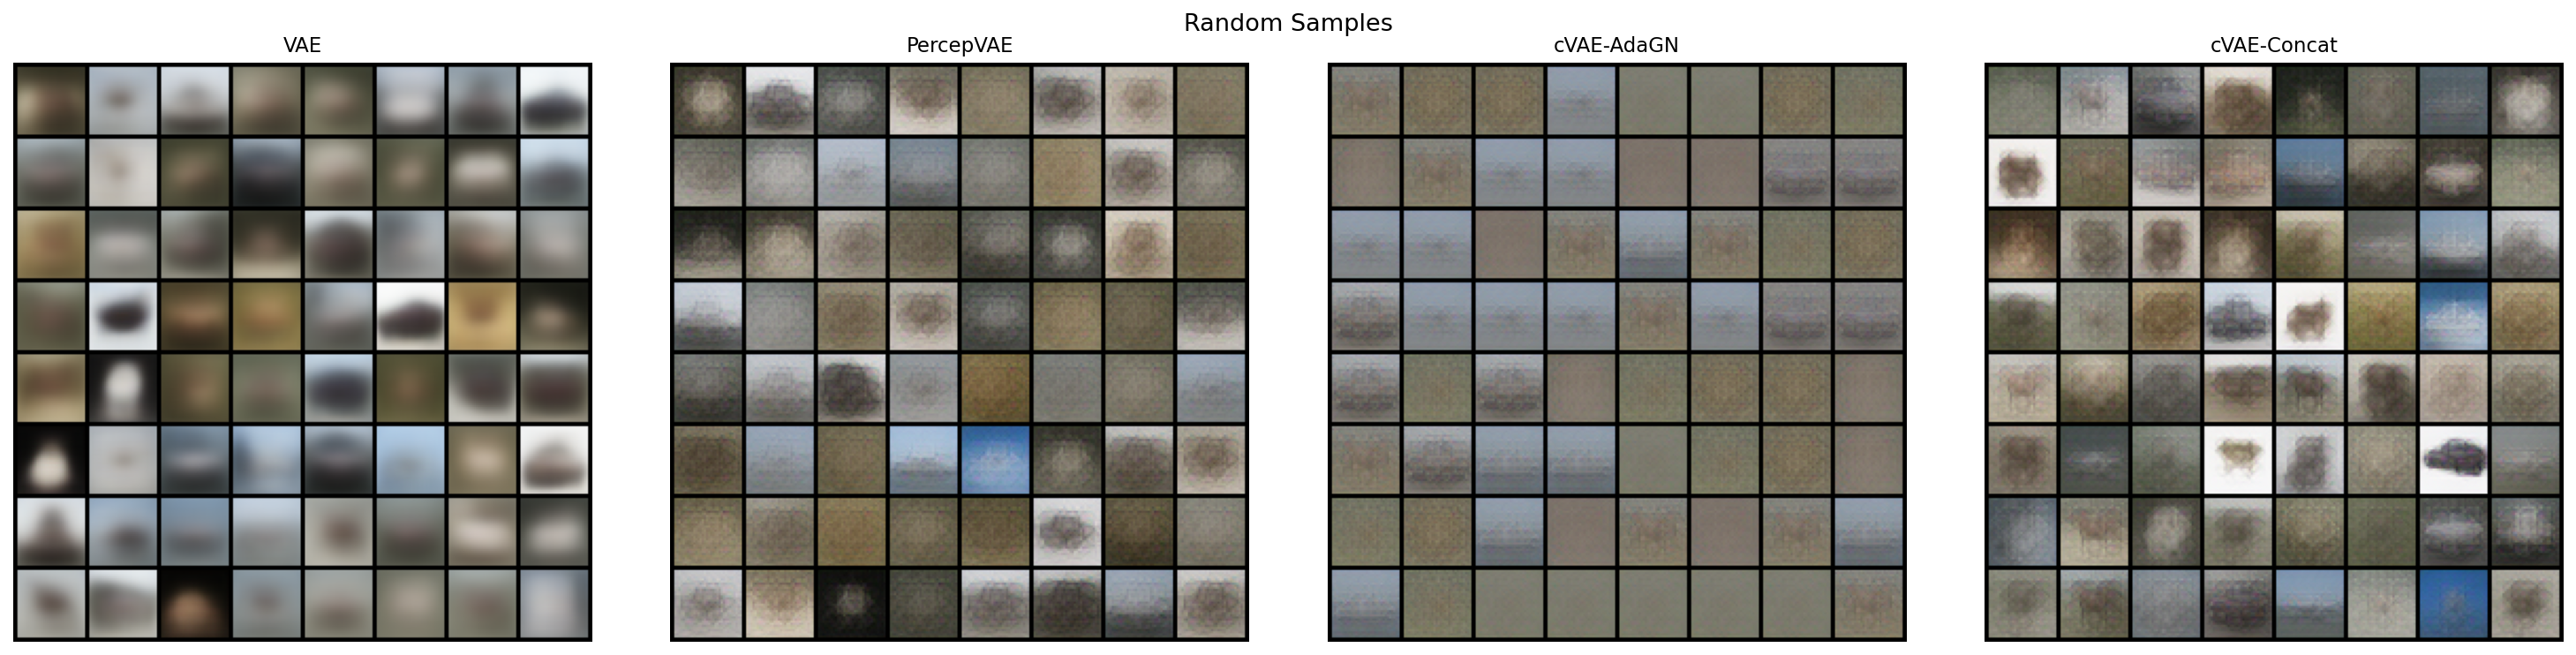
\includegraphics[width=\linewidth]{./with_KL_equals_1/samples.png}
	\caption{Experiment 1 — Randomly sampled images generated by
		decoding latent vectors $\mathbf{z} \sim \mathcal{N}(0,I)$.}
	\label{fig:exp1-samples}
\end{figure}

\subsubsection{Reconstructions}

\begin{figure}[H]
	\centering
	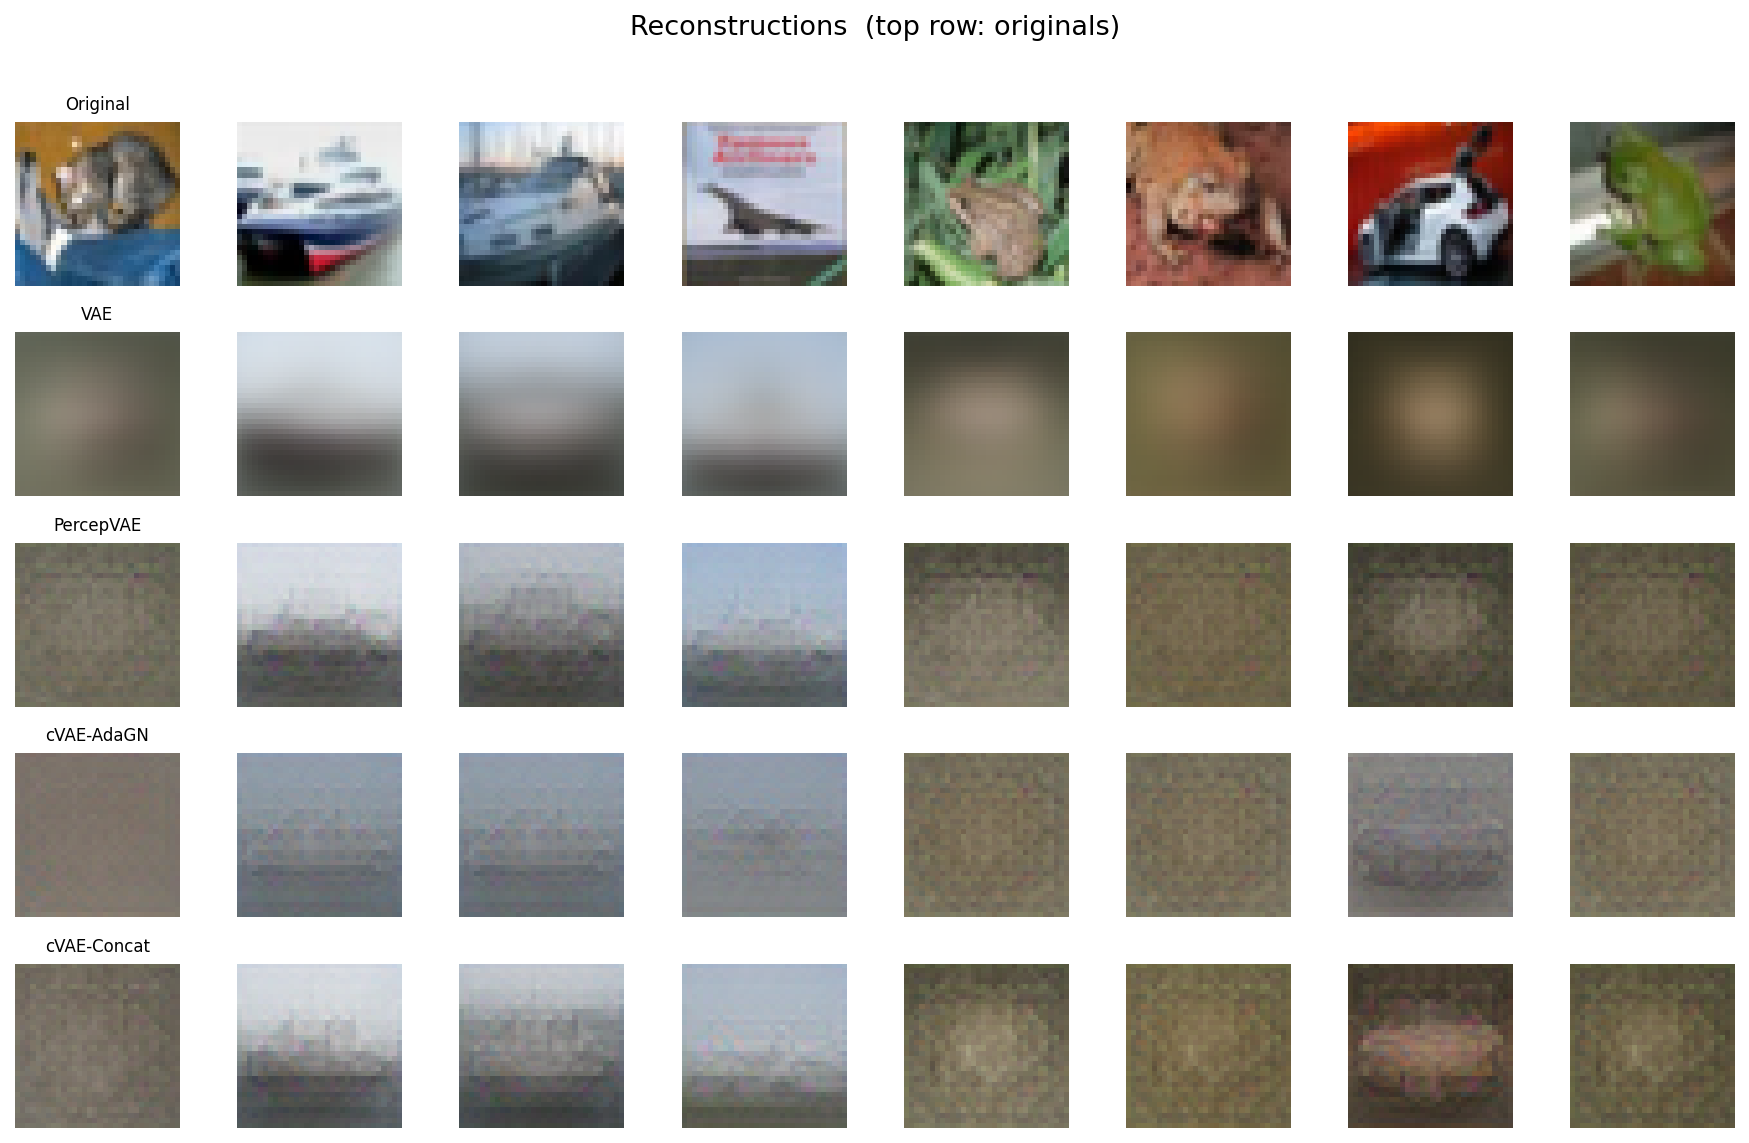
\includegraphics[width=\linewidth]{./with_KL_equals_1/reconstructions.png}
	\caption{Experiment 1 — Input images (top row) and their
		reconstructions (bottom row). Reconstruction quality is
		noticeably better than free generation, reflecting the
		encoder's ability to infer informative posterior means.}
	\label{fig:exp1-recon}
\end{figure}

\subsubsection{Latent-Space Interpolations}

\begin{figure}[H]
	\centering
	\begin{subfigure}[t]{0.48\linewidth}
		\centering
		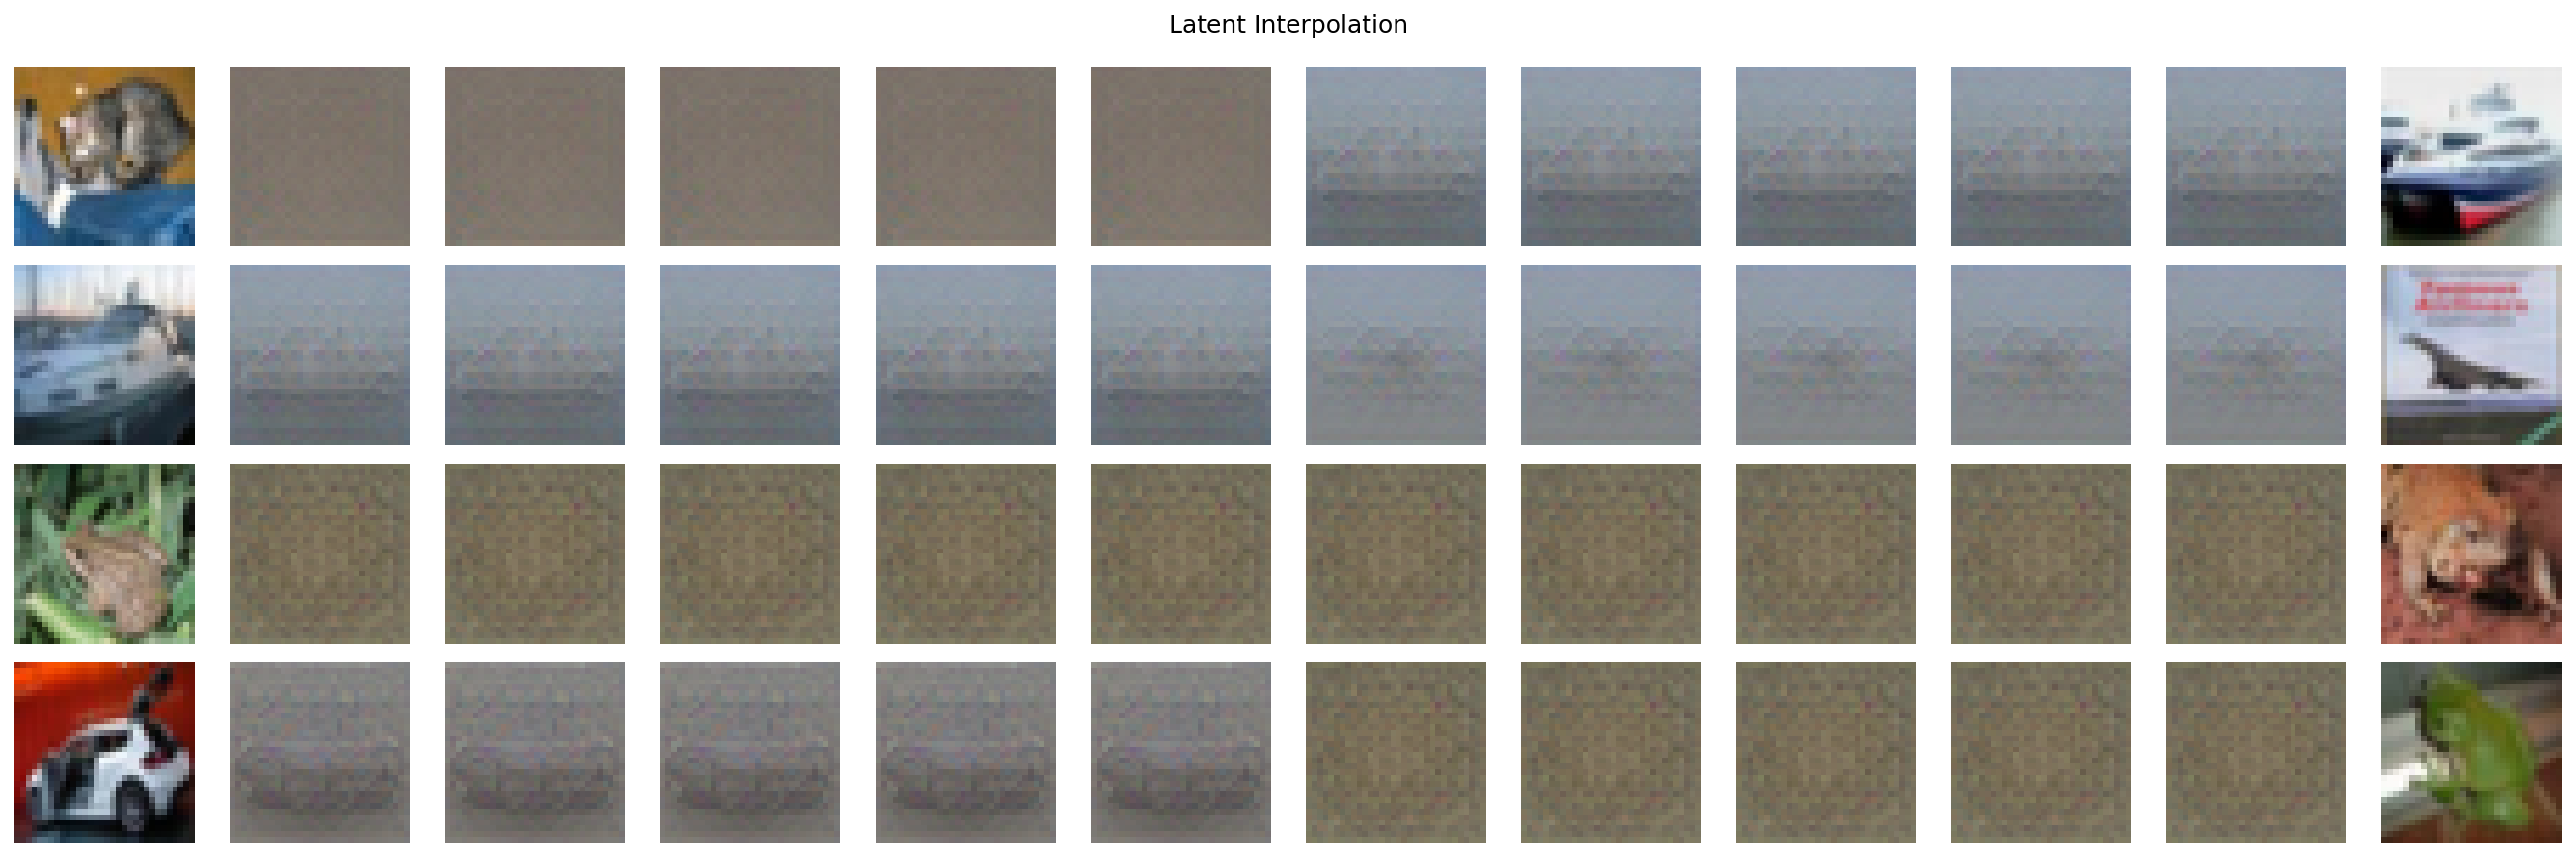
\includegraphics[width=\linewidth]{./with_KL_equals_1/interp_cvae.png}
		\caption{Interpolation For CVAE-AdaGN.}
	\end{subfigure}
	\hfill
	\begin{subfigure}[t]{0.48\linewidth}
		\centering
		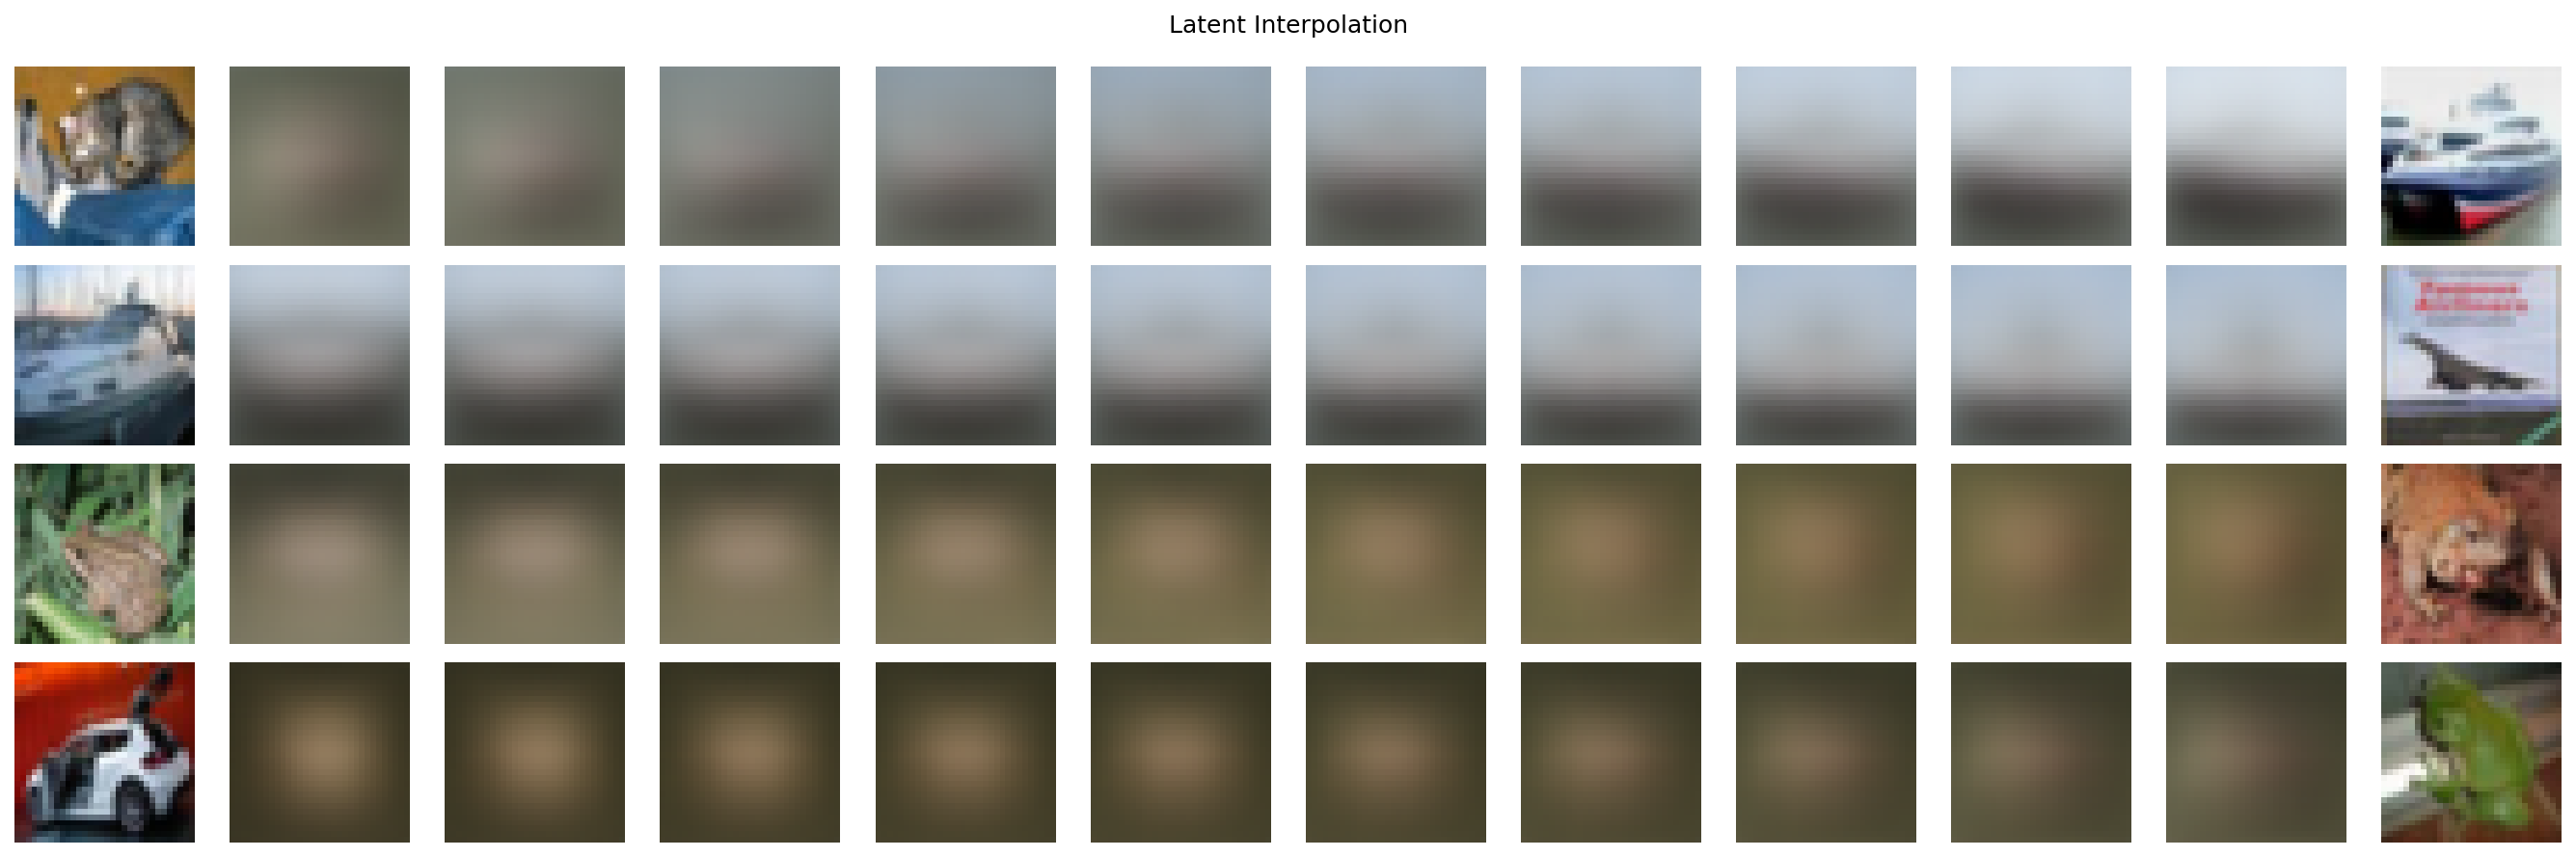
\includegraphics[width=\linewidth]{./with_KL_equals_1/interp_vae.png}
		\caption{Interpolation For Vanilla VAE.}
	\end{subfigure}
	\caption{Experiment 1 — linear interpolation
		between pairs of encoded images in latent space.}
	\label{fig:exp1-interp}
\end{figure}

\subsubsection{Latent-Space Visualisation}

\begin{figure}[H]
	\centering
	\begin{subfigure}[t]{0.31\linewidth}
		\centering
		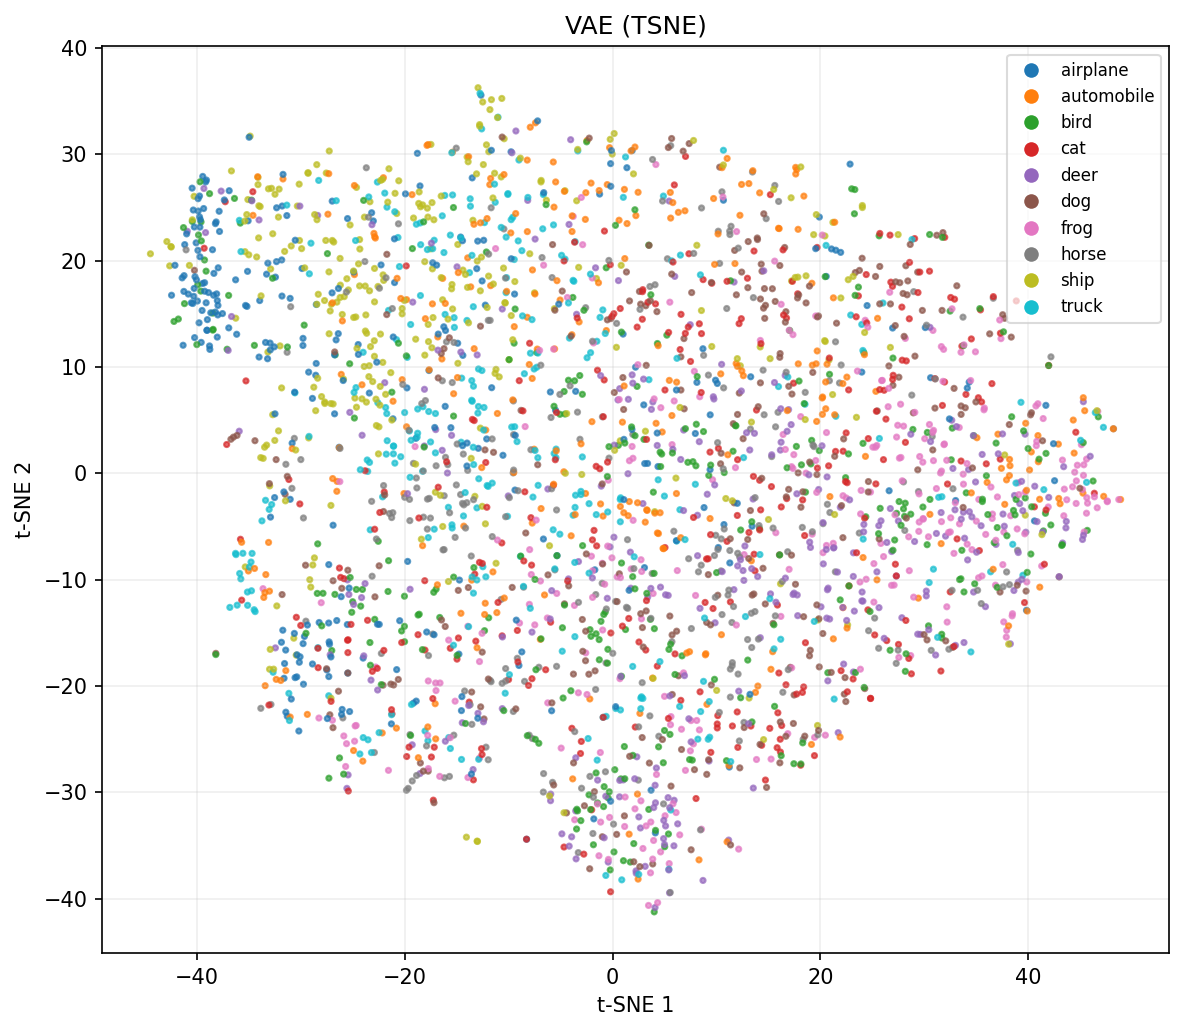
\includegraphics[width=\linewidth]{./with_KL_equals_1/latent_vae.png}
		\caption{VAE}
	\end{subfigure}
	\hfill
	\begin{subfigure}[t]{0.31\linewidth}
		\centering
		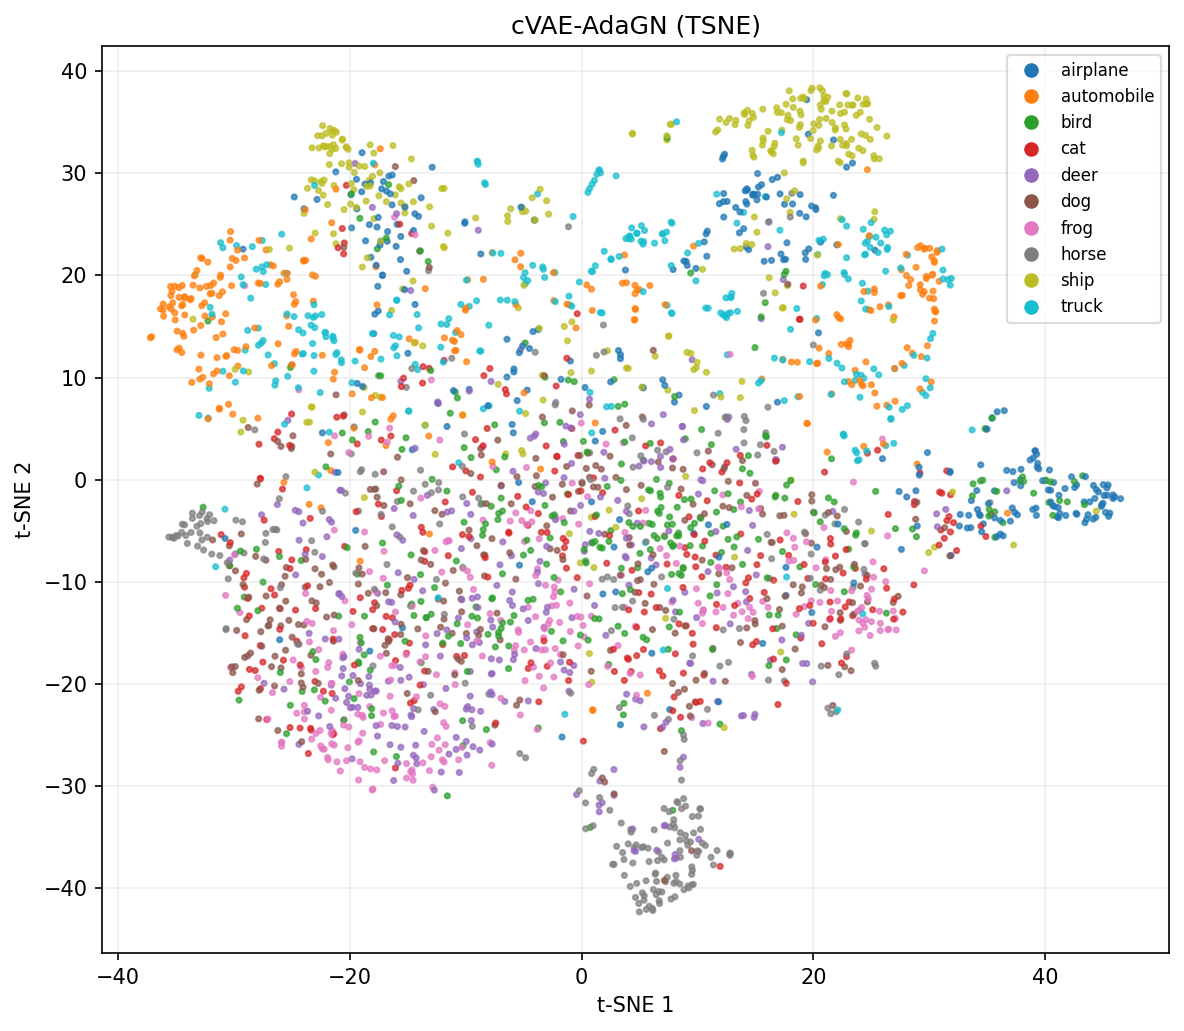
\includegraphics[width=\linewidth]{./with_KL_equals_1/latent_cvae_adagn.png}
		\caption{cVAE-AdaGN}
	\end{subfigure}
	\hfill
	\begin{subfigure}[t]{0.31\linewidth}
		\centering
		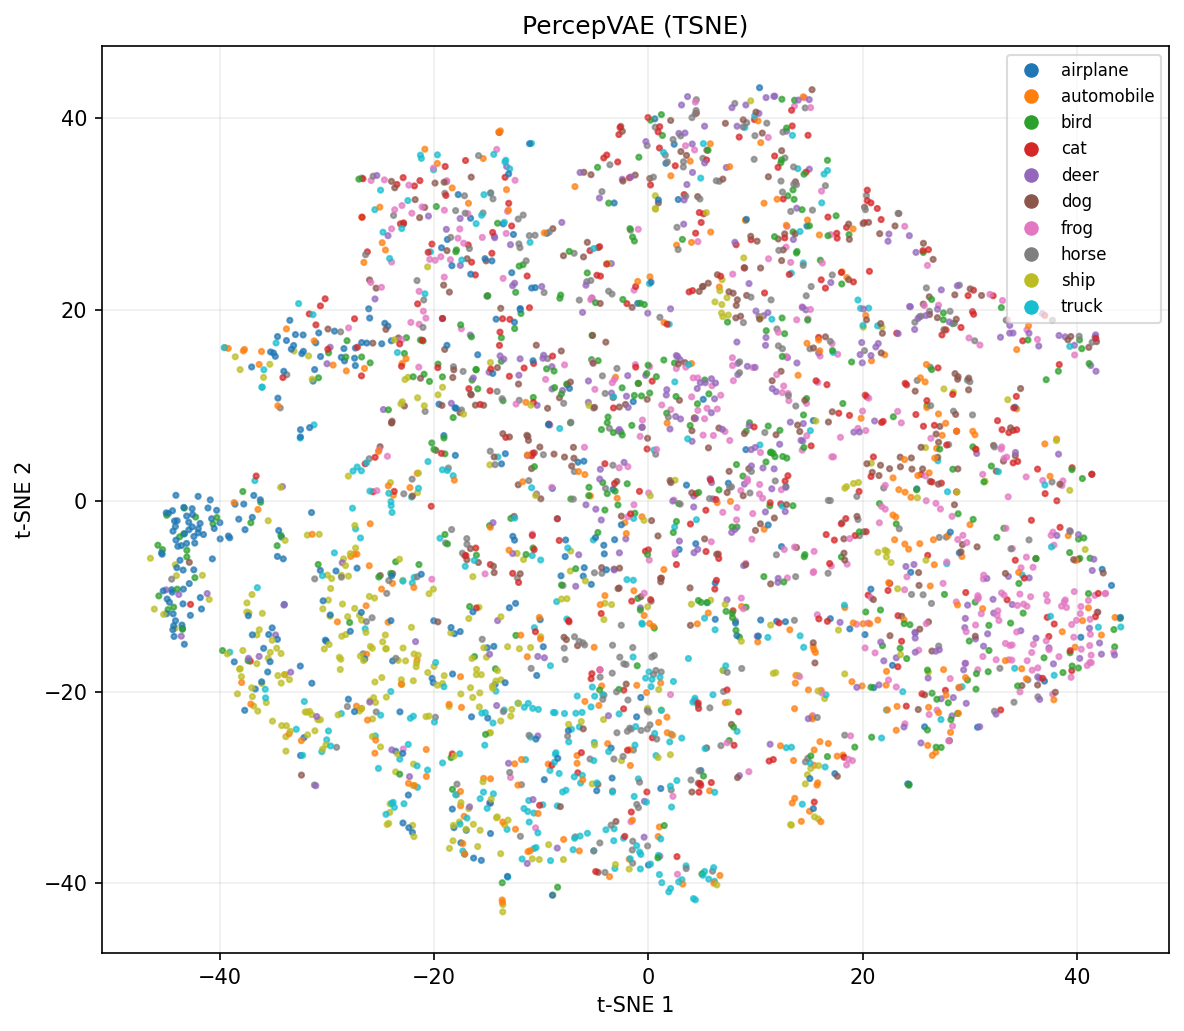
\includegraphics[width=\linewidth]{./with_KL_equals_1/latent_percepvae.png}
		\caption{Perceptual VAE}
	\end{subfigure}
	\caption{Experiment 1 — 2-D t-SNE projections of the latent
		space, coloured by class label.  Tighter, better-separated
		clusters indicate that the model has learned
		class-discriminative structure in $\mathbf{z}$.}
	\label{fig:exp1-latent}
\end{figure}

\subsection{Analysis and Observations}
\label{subsec:exp1-analysis}

\begin{itemize}
	\item \textbf{Conditioning is decisive.} Both cVAE variants
	outperform the unconditional baselines by a substantial margin,
	with cVAE-Concat achieving the lowest FID (163.23) and the
	highest IS (3.54).
	
	\item \textbf{Perceptual loss provides moderate benefit.}
	PercepVAE reduces FID by $\approx$20 points vs.\ the vanilla
	VAE, but its IS slightly decreases, suggesting that perceptual
	regularisation may introduce a diversity-quality trade-off.
	
	\item \textbf{AdaGN vs.\ Concat.} cVAE-Concat outperforms
	cVAE-AdaGN on both FID and IS, indicating that direct feature
	concatenation is a more effective conditioning mechanism than
	normalisation-layer modulation at this scale.
	
	\item \textbf{Reconstruction vs.\ generation gap.}
	Reconstruction quality is visually good (see
	Figure~\ref{fig:exp1-recon}), while free-sampling quality
	remains limited (Figure~\ref{fig:exp1-samples}). This
	posterior-prior gap is a well-known VAE limitation.
	
	\item \textbf{Latent structure.} The t-SNE plots
	(Figure~\ref{fig:exp1-latent}) show that conditional model
	form tighter, more separable clusters, consistent with
	improved IS scores.
\end{itemize}



% ============================================================
\section{Experiment 3}
\label{sec:exp1}

\subsection{Motivation}
\label{subsec:exp1-motivation}

The first experiment establishes the \textbf{baseline} performance of
four VAE variants that differ in their conditioning and loss strategy,
without self-attention. This provides a reference point for subsequent
ablations.

\subsection{Hyperparameters}
\label{subsec:exp1-hp}

\begin{configbox}[Experiment 1 — Variable Hyperparameters]
	\begin{lstlisting}[language=Python, numbers=none]
		{
			"epochs"        : 30,
			"kl_weight"     : .1,   # Weight on KL-divergence term
			"percep_weight" : 0.1,     # Weight on perceptual loss
			"use_attention" : false,   # Self-attention disabled
			"attn_heads"    : 1,
		}
	\end{lstlisting}
\end{configbox}



\subsection{Evaluation Results}
\label{subsec:exp1-results}

\begin{table}[H]
	\centering
	\caption{Experiment 1 — Quantitative evaluation (FID and IS).
		FID: lower is better; IS: higher is better.}
	\label{tab:exp1-metrics}
	\begin{tabular}{lccc}
		\toprule
		\textbf{Model} & \textbf{FID}~$\downarrow$
		& \textbf{IS mean}~$\uparrow$
		& \textbf{IS std} \\
		\midrule
		VAE            & 326.79 & 1.69 & 0.03 \\
		PercepVAE      & 276.51 & 2.22 & 0.06 \\
		cVAE-AdaGN     & 394.40 & 2.03 & 0.03 \\
		cVAE-Concat    & 193.62 & 3.41 & 0.12 \\
		\bottomrule
	\end{tabular}
\end{table}

\subsection{Training Dynamics}
\label{subsec:exp1-training}

\begin{figure}[H]
	\centering
	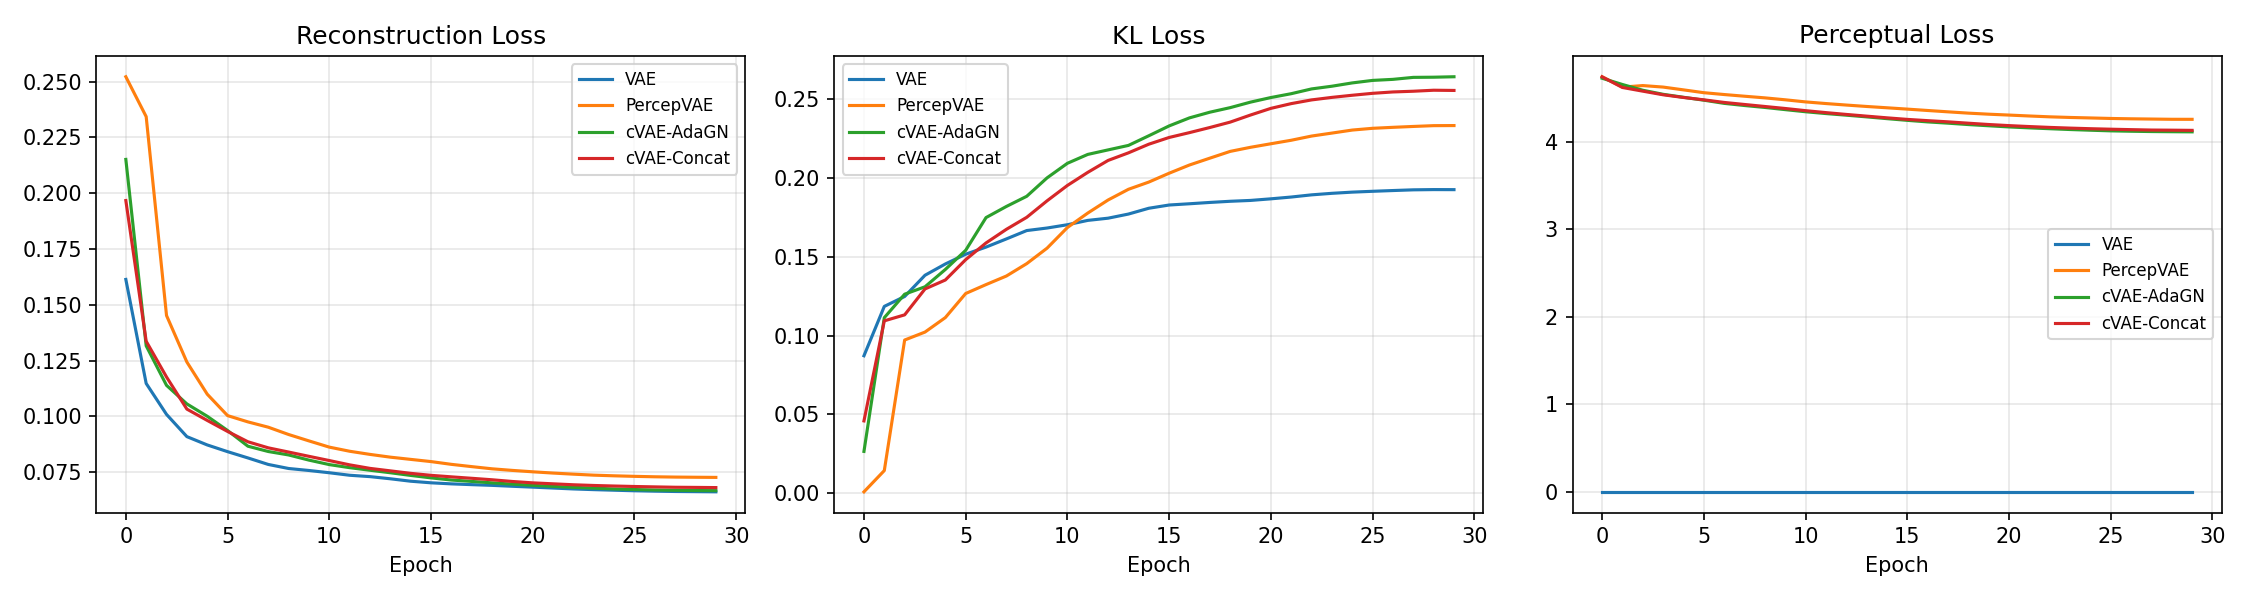
\includegraphics[width=\linewidth]{./with_KL_equals_one_over_ten_and_30_epoch/training_curves.png}
	\caption{Experiment 1 — Training loss curves for all four VAE
		variants. The plot shows the evolution of the total
		loss, reconstruction term, and KL-divergence term over
		50 epochs.}
	\label{fig:exp1-losses}
\end{figure}

\subsection{Qualitative Results}
\label{subsec:exp1-qual}

\subsubsection{Random Samples}

\begin{figure}[H]
	\centering
	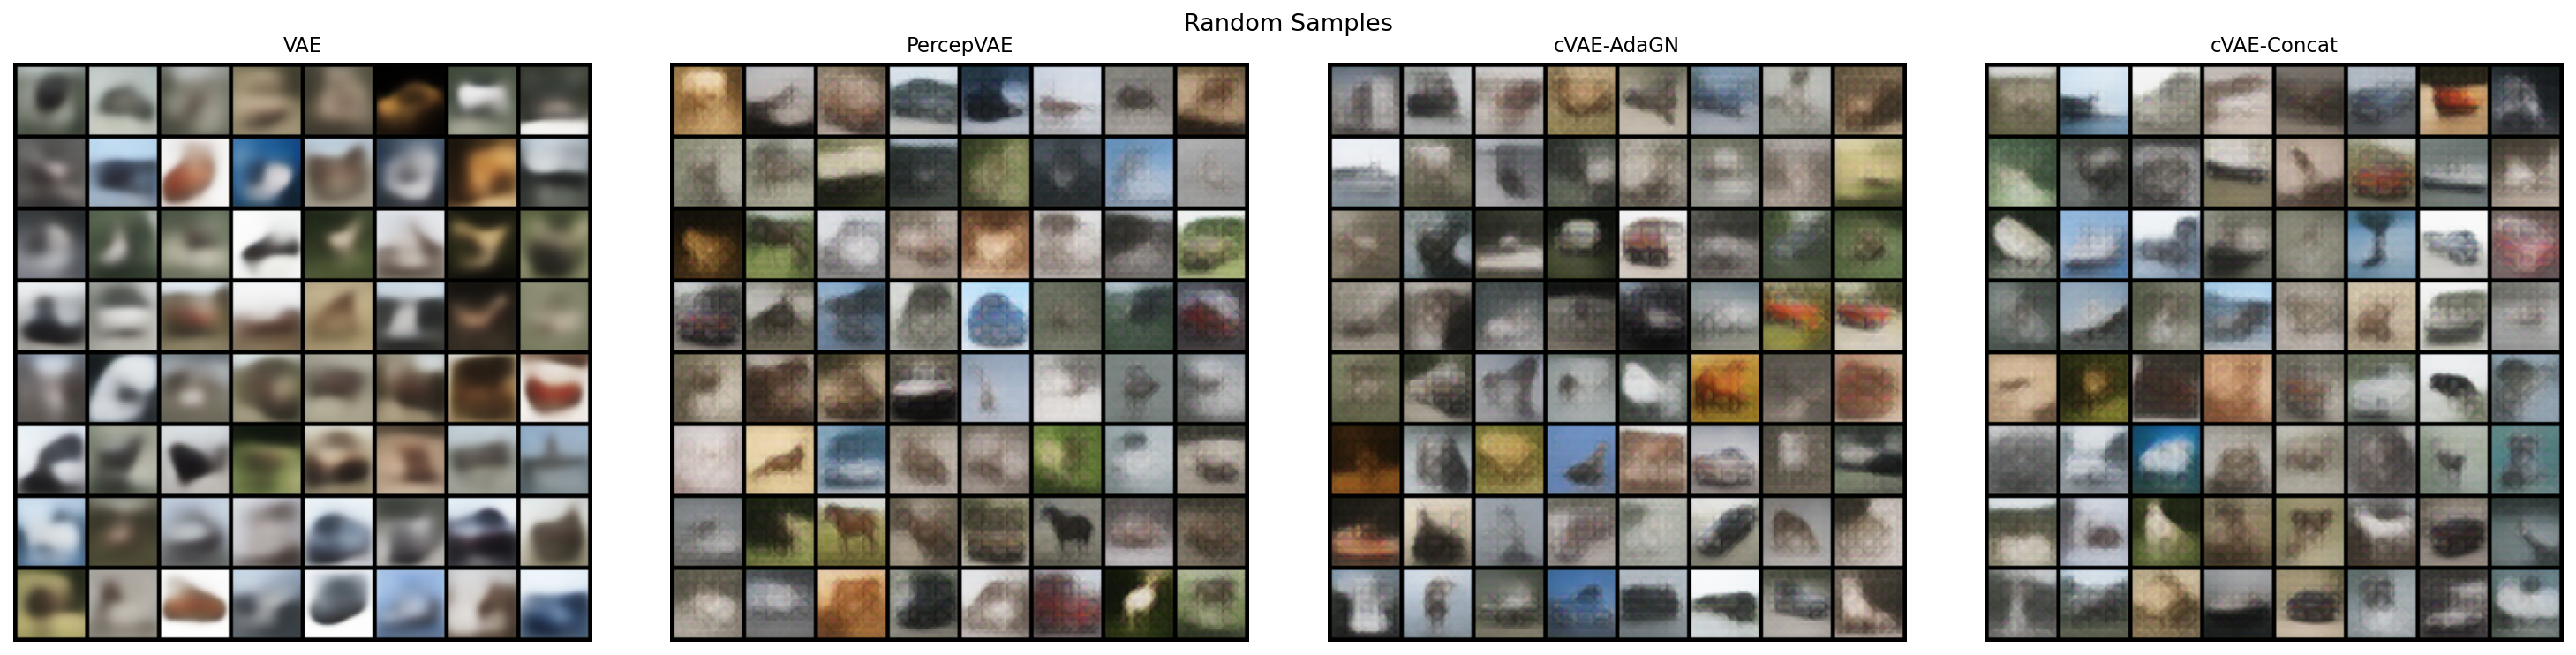
\includegraphics[width=\linewidth]{./with_KL_equals_one_over_ten_and_30_epoch/samples.png}
	\caption{Experiment 1 — Randomly sampled images generated by
		decoding latent vectors $\mathbf{z} \sim \mathcal{N}(0,I)$.}
	\label{fig:exp1-samples}
\end{figure}

\subsubsection{Reconstructions}

\begin{figure}[H]
	\centering
	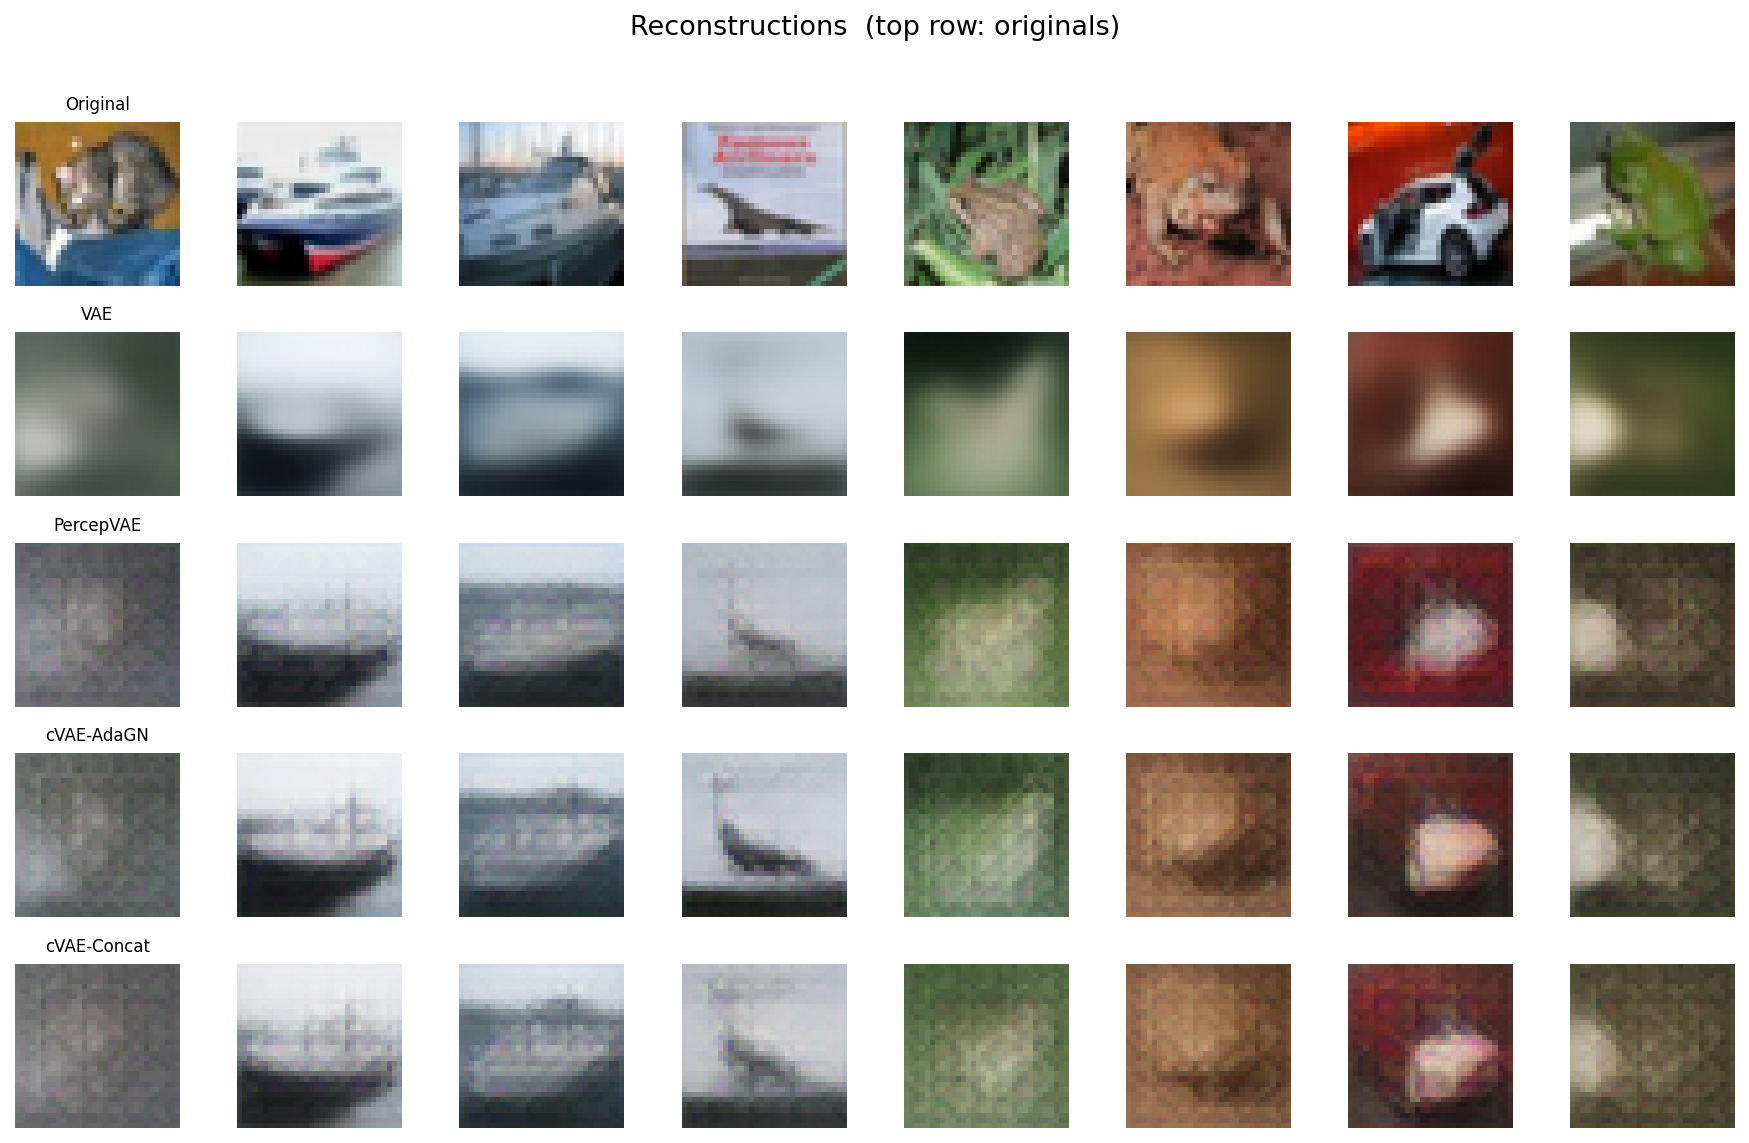
\includegraphics[width=\linewidth]{./with_KL_equals_one_over_ten_and_30_epoch/reconstructions.png}
	\caption{Experiment 1 — Input images (top row) and their
		reconstructions (bottom row). Reconstruction quality is
		noticeably better than free generation, reflecting the
		encoder's ability to infer informative posterior means.}
	\label{fig:exp1-recon}
\end{figure}

\subsubsection{Latent-Space Interpolations}

\begin{figure}[H]
	\centering
	\begin{subfigure}[t]{0.48\linewidth}
		\centering
		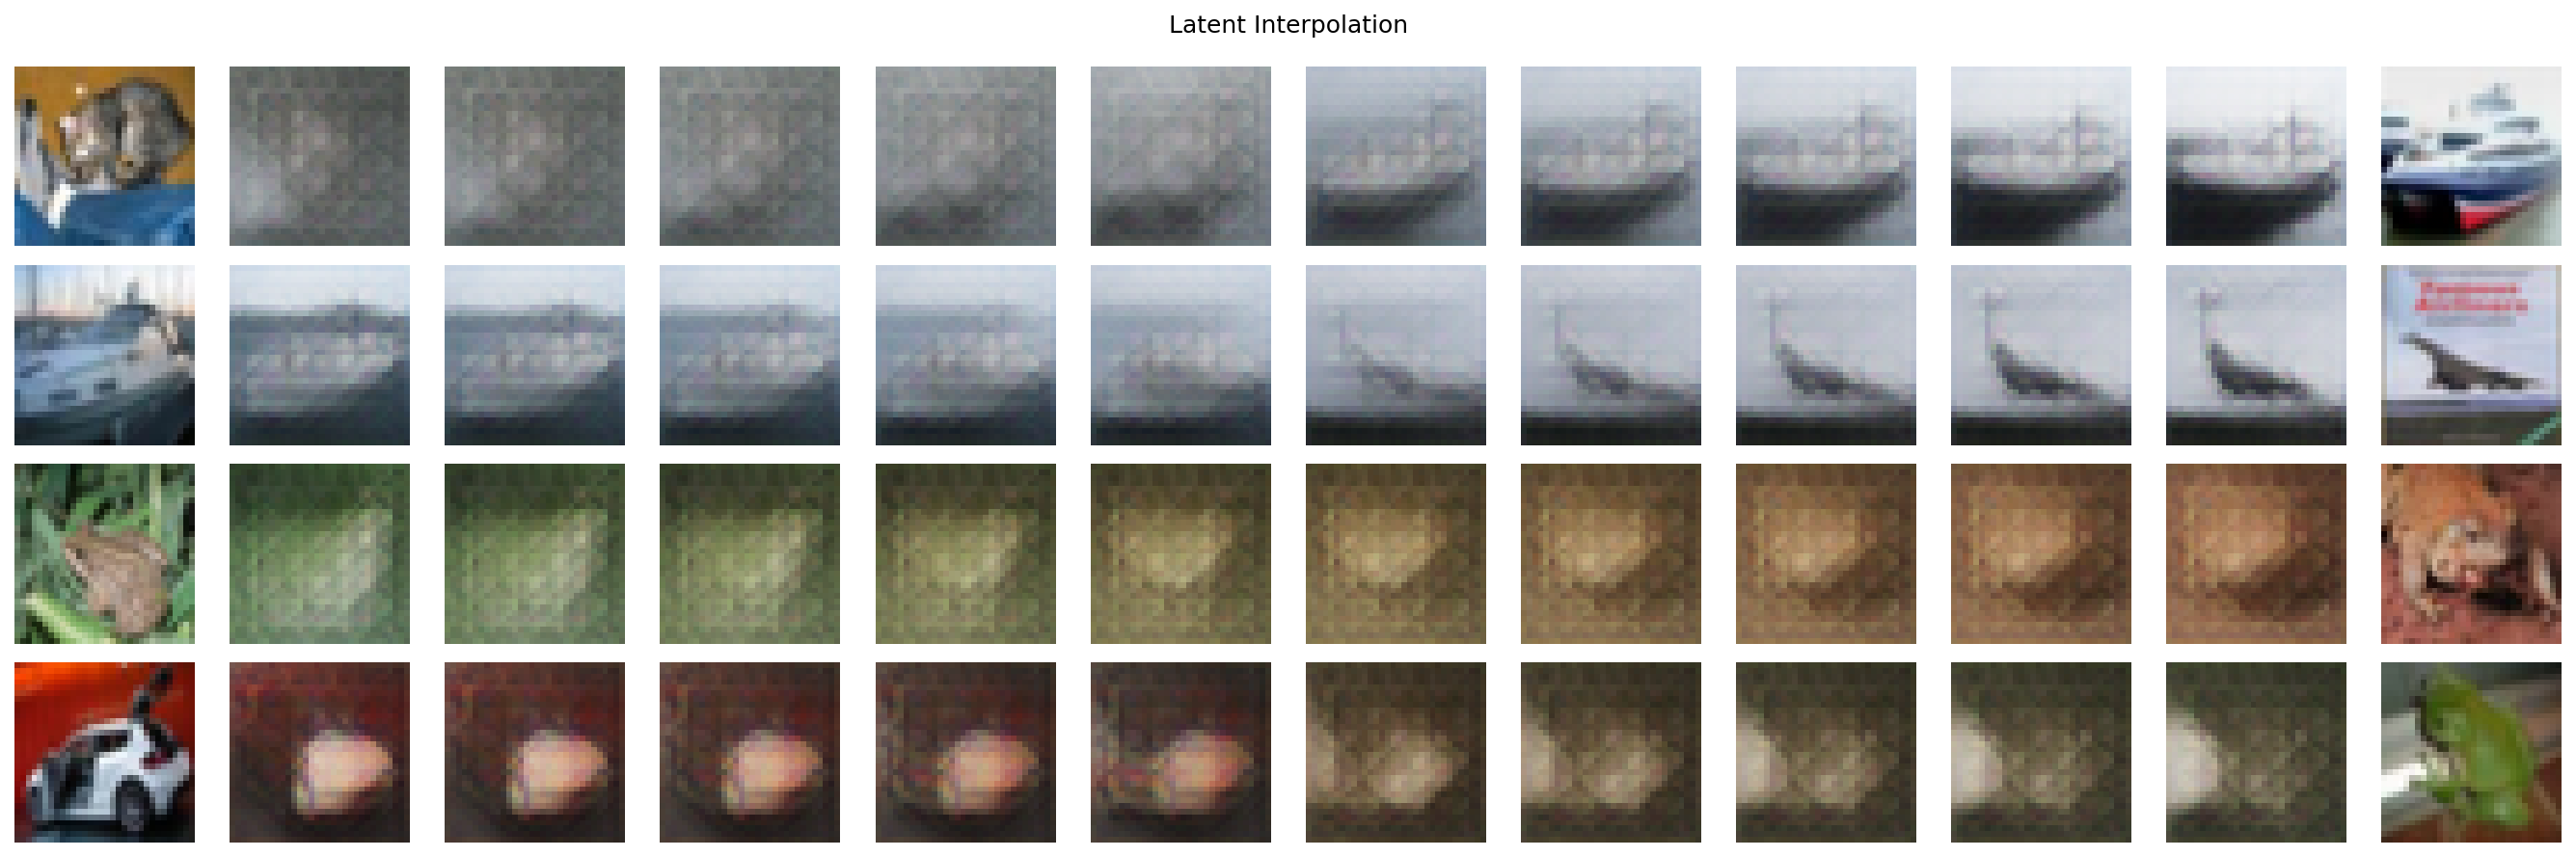
\includegraphics[width=\linewidth]{./with_KL_equals_one_over_ten_and_30_epoch/interp_cvae.png}
		\caption{Interpolation For CVAE-AdaGN.}
	\end{subfigure}
	\hfill
	\begin{subfigure}[t]{0.48\linewidth}
		\centering
		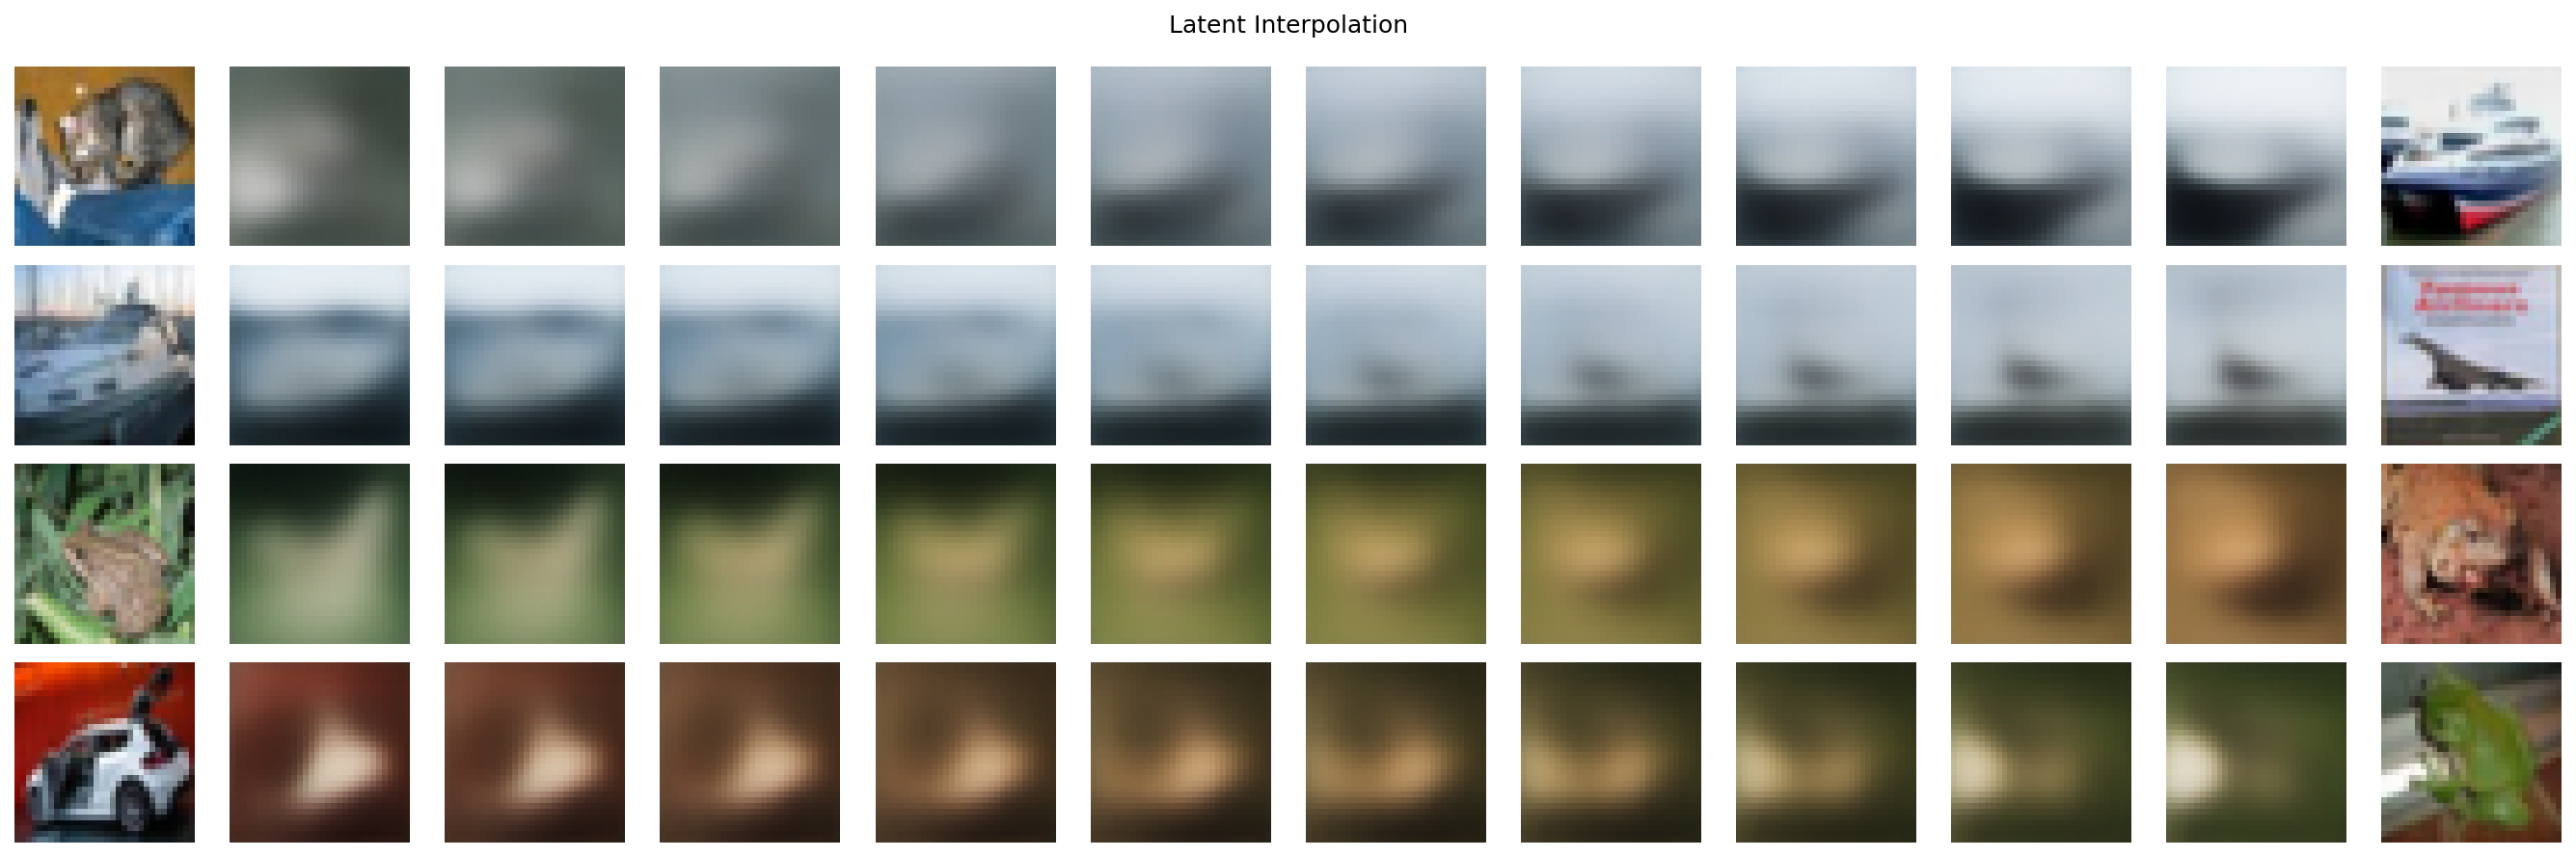
\includegraphics[width=\linewidth]{./with_KL_equals_one_over_ten_and_30_epoch/interp_vae.png}
		\caption{Interpolation For Vanilla VAE.}
	\end{subfigure}
	\caption{Experiment 1 — linear interpolation
		between pairs of encoded images in latent space.}
	\label{fig:exp1-interp}
\end{figure}

\subsubsection{Latent-Space Visualisation}

\begin{figure}[H]
	\centering
	\begin{subfigure}[t]{0.31\linewidth}
		\centering
		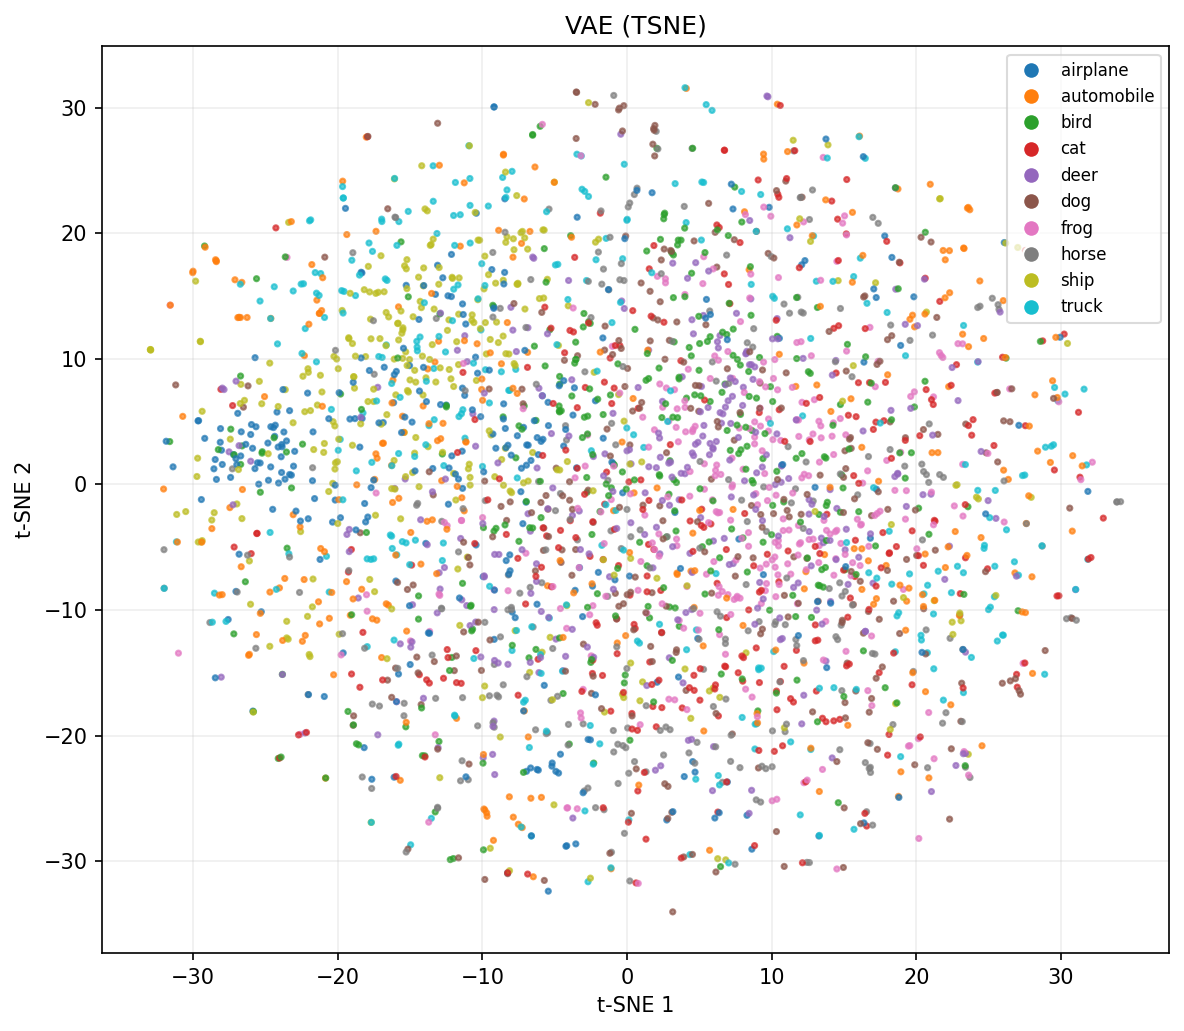
\includegraphics[width=\linewidth]{./with_KL_equals_one_over_ten_and_30_epoch/latent_vae.png}
		\caption{VAE}
	\end{subfigure}
	\hfill
	\begin{subfigure}[t]{0.31\linewidth}
		\centering
		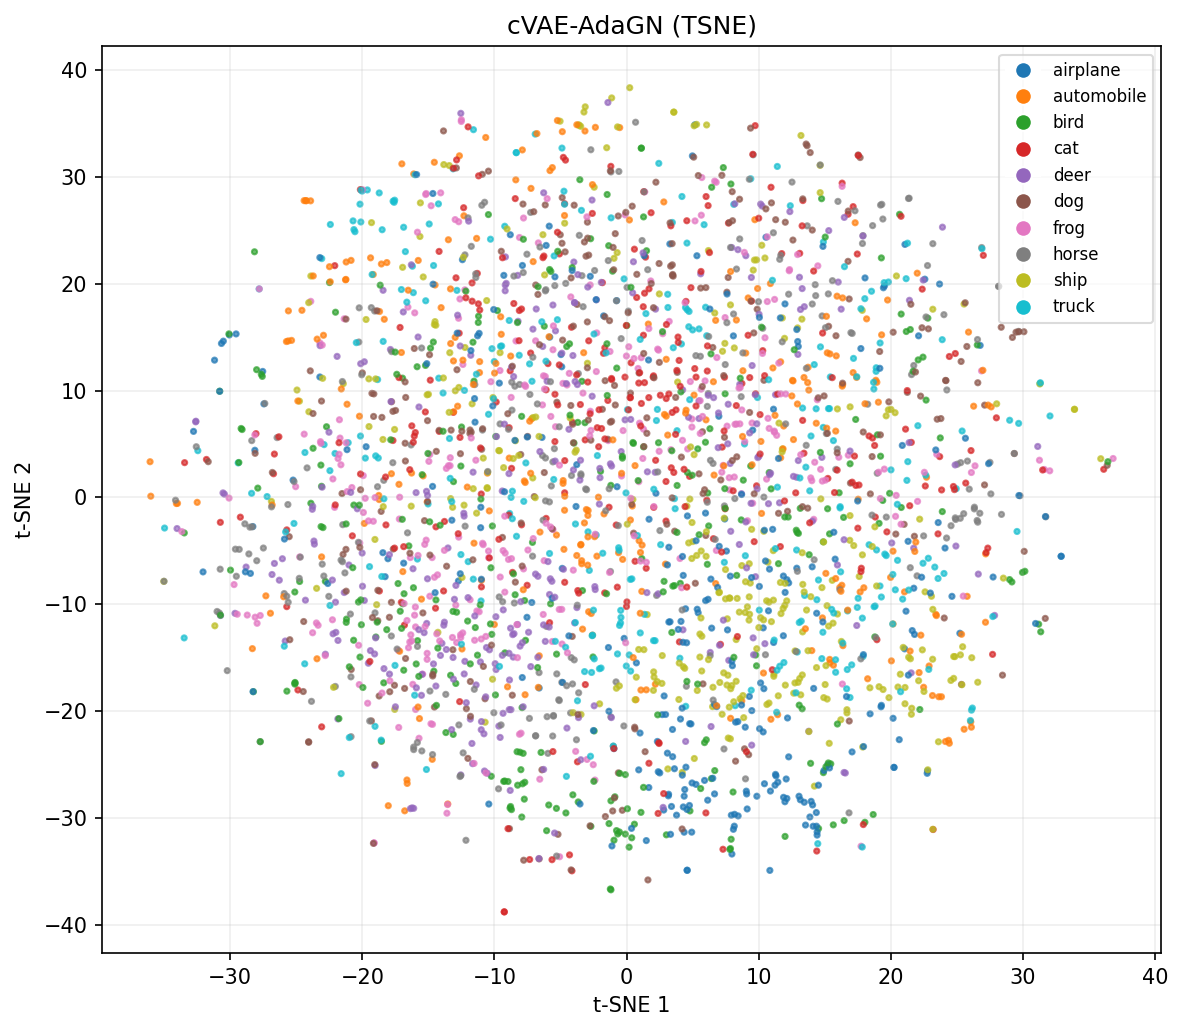
\includegraphics[width=\linewidth]{./with_KL_equals_one_over_ten_and_30_epoch/latent_cvae_adagn.png}
		\caption{cVAE-AdaGN}
	\end{subfigure}
	\hfill
	\begin{subfigure}[t]{0.31\linewidth}
		\centering
		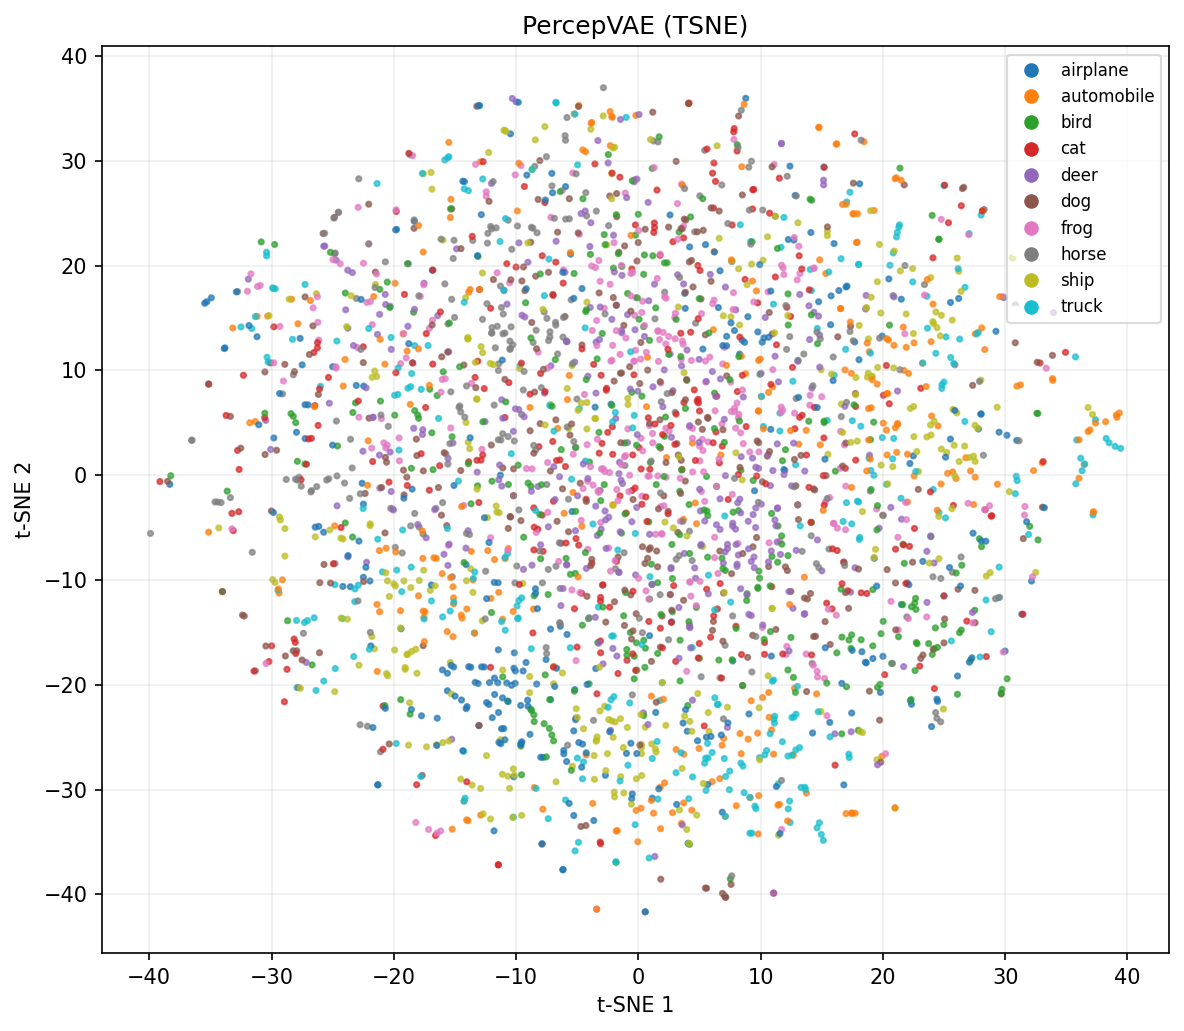
\includegraphics[width=\linewidth]{./with_KL_equals_one_over_ten_and_30_epoch/latent_percepvae.png}
		\caption{Perceptual VAE}
	\end{subfigure}
	\caption{Experiment 1 — 2-D t-SNE projections of the latent
		space, coloured by class label.  Tighter, better-separated
		clusters indicate that the model has learned
		class-discriminative structure in $\mathbf{z}$.}
	\label{fig:exp1-latent}
\end{figure}

\subsection{Analysis and Observations}
\label{subsec:exp1-analysis}

\begin{itemize}
	\item \textbf{Conditioning is decisive.} Both cVAE variants
	outperform the unconditional baselines by a substantial margin,
	with cVAE-Concat achieving the lowest FID (163.23) and the
	highest IS (3.54).
	
	\item \textbf{Perceptual loss provides moderate benefit.}
	PercepVAE reduces FID by $\approx$20 points vs.\ the vanilla
	VAE, but its IS slightly decreases, suggesting that perceptual
	regularisation may introduce a diversity-quality trade-off.
	
	\item \textbf{AdaGN vs.\ Concat.} cVAE-Concat outperforms
	cVAE-AdaGN on both FID and IS, indicating that direct feature
	concatenation is a more effective conditioning mechanism than
	normalisation-layer modulation at this scale.
	
	\item \textbf{Reconstruction vs.\ generation gap.}
	Reconstruction quality is visually good (see
	Figure~\ref{fig:exp1-recon}), while free-sampling quality
	remains limited (Figure~\ref{fig:exp1-samples}). This
	posterior-prior gap is a well-known VAE limitation.
	
	\item \textbf{Latent structure.} The t-SNE plots
	(Figure~\ref{fig:exp1-latent}) show that conditional model
	form tighter, more separable clusters, consistent with
	improved IS scores.
\end{itemize}



% ============================================================
\section{Cross-Experiment Comparison}
\label{sec:cross}

% ── Placeholder ─────────────────────────────────────────────
\begin{tcolorbox}[colback=yellow!8, colframe=orange!60!black,
                  fonttitle=\bfseries, title={Content placeholder}]
Once all VAE experiments are complete, populate the summary table and
figure below.
\end{tcolorbox}

\subsection{Summary Table — All VAE Experiments}

\begin{table}[H]
    \centering
    \caption{Summary of the best-performing VAE variant per experiment.}
    \label{tab:summary}
    \begin{tabularx}{\linewidth}{lXccc}
        \toprule
        \textbf{Exp.} & \textbf{Best Model}
                      & \textbf{Key Change}
                      & \textbf{FID}~$\downarrow$
                      & \textbf{IS}~$\uparrow$ \\
        \midrule
        1 & cVAE-Concat & Conditioning strategy & 163.23 & 3.54 \\
        2 & — & — & — & — \\
        \bottomrule
    \end{tabularx}
\end{table}

\subsection{FID Progression Across Experiments}

\begin{figure}[H]
    \centering
    % \includegraphics[width=0.8\linewidth]{fid_progression.png}
    \caption{FID of the best VAE variant per experiment, showing how
             successive design choices affect generation quality.}
    \label{fig:fid-prog}
\end{figure}

% ============================================================
\section{Conclusions}
\label{sec:conclusions}

% ── Placeholder ─────────────────────────────────────────────
\begin{tcolorbox}[colback=yellow!8, colframe=orange!60!black,
                  fonttitle=\bfseries, title={Content placeholder}]
This section will synthesise:
\begin{itemize}
    \item The most impactful design choices for VAE generation quality
    \item The ceiling on generation quality achievable with the VAE
          objective alone
    \item Key structural properties of the learned latent space
    \item How these findings motivate the comparison with DDPMs
          (addressed in the companion report)
\end{itemize}
\end{tcolorbox}

Based on Experiment~1 alone, several conclusions can already be drawn:

\begin{enumerate}
    \item \textbf{Class conditioning is the single most impactful
          factor} evaluated so far, reducing FID by over 30 points
          relative to the unconditional VAE.

    \item \textbf{Perceptual loss helps FID but not IS}, suggesting
          it encourages more realistic textures at the possible cost of
          diversity.

    \item \textbf{The posterior-prior gap} remains the fundamental
          limitation of VAEs: the model reconstructs well but samples
          poorly. This is structurally different from DDPMs, where
          sampling and generation are the same operation.

    \item \textbf{The latent space is interpretable and smooth}, as
          evidenced by coherent interpolations and class-separable
          t-SNE clusters. This is a property not easily available in
          DDPMs without additional inversion techniques.
\end{enumerate}

% ============================================================
\appendix

\section{Experimental Protocol Checklist}
\label{app:checklist}

Use this checklist when adding a new experiment to the report:

\begin{itemize}[label=$\square$]
    \item State the motivation and hypothesis
    \item List all variable hyperparameters in a \texttt{configbox}
    \item List all model variants with a one-line description each
    \item Include the quantitative results table (FID, IS mean, IS std)
    \item Include the training loss figure
    \item Include the random-samples figure with observation
    \item Include the reconstruction figure with observation
    \item Include the latent-interpolation figure
    \item Include the latent t-SNE visualisation
    \item Write an analysis subsection with bullet-point observations
    \item Update the cross-experiment summary table (Section~\ref{sec:cross})
\end{itemize}

\section{Metric Definitions}
\label{app:metrics}

\paragraph{Fréchet Inception Distance (FID).}
Let $\mu_r, \Sigma_r$ and $\mu_g, \Sigma_g$ be the mean and covariance
of Inception-v3 pool3 features extracted from real and generated
images respectively. Then:
\[
    \mathrm{FID} = \|\mu_r - \mu_g\|^2
                 + \mathrm{tr}\!\left(
                     \Sigma_r + \Sigma_g
                     - 2\!\left(\Sigma_r \Sigma_g\right)^{1/2}
                   \right).
\]

\paragraph{Inception Score (IS).}
\[
    \mathrm{IS} = \exp\!\left(
        \mathbb{E}_{\mathbf{x}}\left[
            D_{\mathrm{KL}}\!\left(
                p(y|\mathbf{x}) \,\|\, p(y)
            \right)
        \right]
    \right),
\]
where $p(y|\mathbf{x})$ is the Inception classifier's conditional
label distribution and $p(y) = \int p(y|\mathbf{x})\,p(\mathbf{x})\,d\mathbf{x}$.

\end{document}
